\documentclass{bmstu}

\usepackage{csvsimple}

\addbibresource{rpz.bib}
% 8 Листинги

\usepackage{slashbox}
\usepackage{multirow}

\usepackage{adjustbox}

\usepackage{listings}

% Значения по умолчанию
\lstset{
  basicstyle= \footnotesize,
  breakatwhitespace=true,% разрыв строк только на whitespacce
  breaklines=true,       % переносить длинные строки
%   captionpos=b,          % подписи снизу -- вроде не надо
  inputencoding=koi8-r,
  numbers=left,          % нумерация слева
  numberstyle=\footnotesize,
  showspaces=false,      % показывать пробелы подчеркиваниями -- идиотизм 70-х годов
  showstringspaces=false,
  showtabs=false,        % и табы тоже
  stepnumber=1,
  tabsize=4,              % кому нужны табы по 8 символов?
  frame=single,
  xleftmargin=2.4em,
  framexleftmargin=2em
}

% Стиль для псевдокода: строчки обычно короткие, поэтому размер шрифта побольше
\lstdefinestyle{pseudocode}{
  basicstyle=\small,
  keywordstyle=\color{black}\bfseries\underbar,
  language=Pseudocode,
  numberstyle=\footnotesize,
  commentstyle=\footnotesize\it
}

% Стиль для обычного кода: маленький шрифт
\lstdefinestyle{realcode}{
  basicstyle=\scriptsize,
  numberstyle=\footnotesize
}

% Стиль для коротких кусков обычного кода: средний шрифт
\lstdefinestyle{simplecode}{
  basicstyle=\footnotesize,
  numberstyle=\footnotesize
}

% Стиль для BNF
\lstdefinestyle{grammar}{
  basicstyle=\footnotesize,
  numberstyle=\footnotesize,
  stringstyle=\bfseries\ttfamily,
  language=BNF
}

% Определим свой язык для написания псевдокодов на основе Python
\lstdefinelanguage[]{Pseudocode}[]{Python}{
  morekeywords={each,empty,wait,do},% ключевые слова добавлять сюда
  morecomment=[s]{\{}{\}},% комменты {а-ля Pascal} смотрятся нагляднее
  literate=% а сюда добавлять операторы, которые хотите отображать как мат. символы
    {->}{\ensuremath{$\rightarrow$}~}2%
    {<-}{\ensuremath{$\leftarrow$}~}2%
    {:=}{\ensuremath{$\leftarrow$}~}2%
    {<--}{\ensuremath{$\Longleftarrow$}~}2%
}[keywords,comments]

% Свой язык для задания грамматик в BNF
\lstdefinelanguage[]{BNF}[]{}{
  morekeywords={},
  morecomment=[s]{@}{@},
  morestring=[b]",%
  literate=%
    {->}{\ensuremath{$\rightarrow$}~}2%
    {*}{\ensuremath{$^*$}~}2%
    {+}{\ensuremath{$^+$}~}2%
    {|}{\ensuremath{$|$}~}2%
}[keywords,comments,strings]

% Подписи к листингам на русском языке.
\renewcommand\lstlistingname{Листинг}
\renewcommand\lstlistlistingname{Листинги}

\newcommand{\specialcell}[2][c]{%
  \begin{tabular}[#1]{@{}c@{}}#2\end{tabular}}
  
\def\labelitemi{---}

\newcommand*{\undertext}[2]{%
  \begin{tabular}[t]{@{}c@{}}%
    #1\\\relax\scriptsize(#2)%
  \end{tabular}
}

\usepackage{ctable}% http://ctan.org/pkg/ctable
\usepackage{caption}% http://ctan.org/pkg/caption
\usepackage{subcaption}
\captionsetup[table]{justification=raggedleft,singlelinecheck=off}

\begin{document}

\makethesistitle{Информатика и системы управления}{Программное обеспечение ЭВМ и информационные технологии}{Метод восстановления дефокусированных изображений на основе определенных параметров искажения}{ИУ7-86Б}{П.~Ю.~Сироткина}{М.~В.~Филиппов}{}{}{Д.~Ю.~Мальцева}

\setcounter{page}{5}

\begin{essay}{}
    \noindent\textbf{Ключевые слова}: цифровое изображение, преобразование Фурье, искажение, дефокусировка, размытие, функция рассеяния точки, конволюция, <<слепая>> деконволюция, спектр, кепстр.

    Объектом исследования является цифровое изображение, искаженное дефокусировкой фотокамеры.
    
    Целью работы являлась разработка метода восстановления дефокусированных изображений на основе определенных параметров искажения. 
    
    Для достижения поставленной цели были решены следующие задачи:
    
    \begin{itemize}
    	\item[---] проведен анализ предметной области восстановления дефокусированных изображений;
    	\item[---] проведен сравнительный анализ методов восстановления без учета априорной информации об искажении;
    	\item[---] разработан метод восстановления дефокусированных изображений на основе определенных параметров искажения;
    	\item[---] спроектировано и реализовано программное обеспечение для реализации разрабатываемого метода;
    	\item[---] разработанный метод исследован на применимость при работе с различными типами дефокусированных изображений. 
    \end{itemize}
    
    Разработанный метод имеет ряд ограничений, однако может быть применим даже в условиях отсутствия априорной информации об искажающем процессе.
    
    Было выявлено, что зависимость времени обработки изображения от его размера и цветовой модели имеет линейный вид, а обработка цветного изображения в среднем требует примерно в 3 раза больше времени, чем обработка серого. 
    
    Была определена область применимости предложенного метода: в диапазоне радиуса дефокусировки от 10 до 20 единиц точность восстановления является удовлетворительный, а в случае обработки серого изображения этот диапазон еще шире, поэтому если учет информации о цвете изображения некритичен, то рекомендуется использовать серое изображение вместо цветного в целях сокращения времени обработки и повышения качества результата.
    
    В качестве перспектив дальнейшего развития реализованного программного обеспечения можно рассмотреть учет сложных моделей дефокусировки, возникающих в реальных условиях, применимость к видеофайлам, а также адаптацию предложенного решения под другие языки программирования в целях достижения независимости и кроссплатформенности.
\end{essay}

\maketableofcontents

\begin{abbreviations}
	\definition{\textbf{ФРТ}}{функция рассеяния точки (PSF, Point Spread Function).}
    \definition{\textbf{Спектр}}{результат применения преобразования Фурье к сигналу.}
	\definition{\textbf{Кепстр}}{результат применения преобразования Фурье к логарифму амплитудного спектра.}
	\definition{\textbf{Конволюция}}{операция в функциональном анализе, которая при применении к двум функциям $f$ и $g$ возвращает третью функцию, соответствующую взаимнокорреляционной функции $f(x)$ и $g(-x)$.}
	\definition{\textbf{Деконволюция}}{операция, обратная конволюции.}
    \definition{\textbf{Классическая деконволюция}}{деконволюция изображения на основе априорной информации об искажении.}
    \definition{\textbf{Слепая деконволюция}}{деконволюция изображения без учета априорной информации об искажении.}
	\definition{\textbf{PSNR (англ. Peak Signal-to-Noise Ratio)}}{пиковое отношение сигнал~--~шум.}
\end{abbreviations}
\chapter*{ВВЕДЕНИЕ}
\addcontentsline{toc}{chapter}{ВВЕДЕНИЕ}

Среди способов восприятия человеком информации об окружающем мире посредством органов чувств зрение занимает особое место --- с помощью глаз в среднем воспринимается до 80~\% информации, поступающей из внешней среды.~\cite{percent} Именно поэтому зрительные образы, часто запечатляемые снимками фотокамеры, играют важнейшую роль в нашей жизни. 

Системы фотосъемки могут быть использованы в различных сферах деятельности: криминалистика, кинематография, микроэлектроника, биомедицина, археология, исследования космоса, оборонное производство.~\cite{spheres}

Однако часто полученный снимок фотокамеры оказывается искаженным за счет различных причин: шумы, элементы интерференции и размытие, вызванное дефокусировкой, движением и нелинейностью пленки.~\cite{damage}

Целью данной научно-исследовательской работы является изучение и классификация известных методов восстановления изображений, искаженных дефокусировкой фотокамеры.

Для достижения поставленной цели необходимо выполнить следующие задачи:

\begin{itemize}
	\item провести анализ предметной области восстановления изображений, искаженных дефокусировкой фотокамеры;
	\item провести обзор существующих методов восстановления изображений, искаженных дефокусировкой фотокамеры;
	\item сформулировать критерии сравнения рассмотренных методов;
	\item классифицировать рассмотренные методы;
	\item на основе полученных теоретических сведений сделать выводы.
\end{itemize}
\chapter{Анализ предметной области}
\label{cha:analysis}

\section{Фотокамера}

Фотокамера (фотоаппарат) --- это прибор для получения на фотографическом материале действительного изображения предмета при фотографировании.~\cite{gost}

Цифровой фотоаппарат --- фотоаппарат, в котором для регистрации изображения используется фотоэлектрический принцип. В данной научно-исследовательской работе рассматривается этот тип фотоаппаратов в виду их повсеместного использования и универсальности. 

На рисунке 1.1 представлены основные элементы цифрового фотоаппарата.

\begin{figure}[!h]
	\center{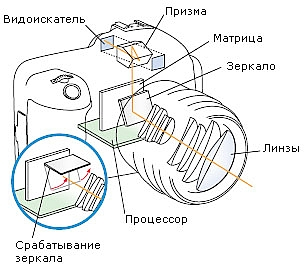
\includegraphics[scale=0.8]{assets/camera}}
	\caption{Основные элементы цифрового фотоаппарата}
\end{figure}

Кратко принцип работы цифрового фотоаппарата можно описать следующим образом: фотон попадает на светочувствительную матрицу, световая энергия преобразуется в электрическую, которая посредством дискретизации и квантования напряжения преобразует энергию в цифровые данные, которые в дальнейшем хранятся в памяти некоторой вычислительной машины с энергонезависимым запоминающим устройством.

В рамках данной работы наибольший интерес представляет фотоматрица --- специализированная аналоговая или цифро-аналоговая интегральная микросхема, состоящая из светочувствительных элементов (фотосенсоров). Матрица предназначена для преобразования спроецированного на нее оптического изображения в аналоговый сигнал (или в набор цифровых данных, если в матрице присутствует аналого-цифровой преобразователь).

\section{Цифровое изображение}

Изображение, получаемое фотокамерой, можно определить как двумерную функцию $f(x,\;y)$, где $x$ и $y$ --- пространственные координаты. Значение функции $f$ в некоторой точке, задаваемой парой координат $(x,\;y)$, является положительной скалярной величиной, называемой интенсивностью, или яркостью изображения в этой точке.~\cite{gonsales}

Для изображений, получаемых \textit{цифровой} фотокамерой, величины $x, y$ и $f$ принимают конечное число дискретных значений. Такие изображения называются цифровыми.

Модель процесса получения дефокусированного цифрового изображения в пространственной области может быть представлена в виде выражения~(1.1)~\cite{defocus_model}:

\begin{equation}
	g(x,\;y) = f(x,\;y) \oplus h(x,\;y) + \eta(x,\;y),
\end{equation}

где: 

\begin{itemize}
	\item $f(x,\;y)$ --- функция, описывающая исходное изображение (неискаженное);
	\item $g(x,\;y)$ --- функция, описывающее дефокусированное изображение (искаженное);
	\item $h(x,\;y)$ --- функция размытия точки (или оптическая передаточная функция), или ядро искажающего оператора \cite{frt};
	\item $\eta(x,\;y)$ --- функция шума;
	\item символ <<$\oplus$>> --- оператор свертки.
\end{itemize}

Задача восстановления изображения заключается в поиске наилучшего приближения $\hat{f}(x,\;y)$ исходного изображения.

\subsection*{Cвертка (конволюция)}

Применительно к обработке цифровых изображений операция свертки может быть интерпретирована следующим образом: на основе некоторого множества пикселей в исходном изображении вычисляется новый пиксель результирующего (искаженного ядром свертки) изображения.

На рисунке 1.4 представлен пример выполнения операции свертки. Для вычисления новых значений используется т.~н. ядро свертки: на приведенном рисунке ядром является матрица зеленого цвета размером $3\times3$.

%В общем случае применение операции свертки к изображению приводит к уменьшению его размера.

\begin{figure}[!h]
	\center{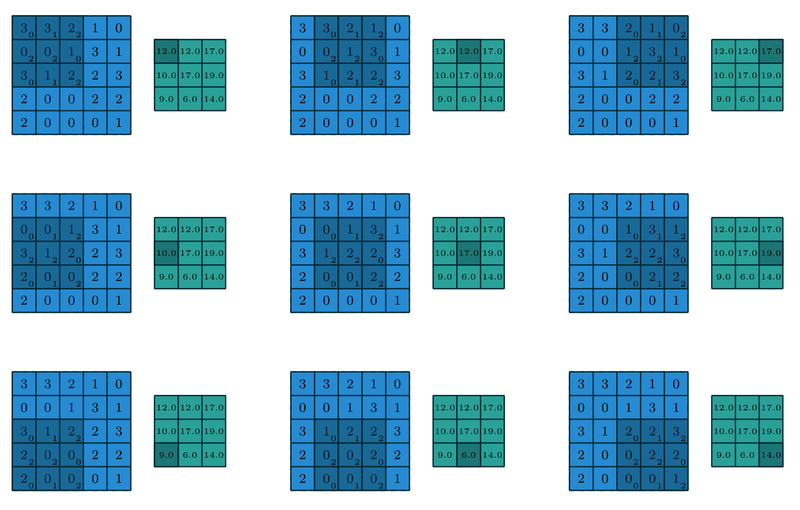
\includegraphics[scale=1.5]{assets/convolution_example}}
	\caption{Пример выполнения операции свертки}
\end{figure}

В зависимости от выбранного ядра свертки, примененного к изображению, можно получить тот или иной эффект: размытость, повышение резкости, обнаружение контуров, граничное обнаружение и др.

Математически операцию двумерной свертки изображения в пространственной области можно описать в виде выражения (1.2).

\begin{equation}
	f(x,\;y) \oplus h(x,\;y) = \sum_{i = -a}^{a} \sum_{j = -b}^{b} f(x + i, y + j) \cdot h(x,\;y),
\end{equation}

где $a = \cfrac{M-1}{2}, b = \cfrac{N-1}{2}$, M, N - размеры изображения,.

Получение функций $f(x,\;y)$ и $h(x,\;y)$ из выражения (1.2) путем выполнения обратных действий приводит к получению большой системы уравнений, решение которой является нетривиальной и трудоемкой задачей.~\cite{teorema} Упростить ее решение может \textit{теорема о свертке}, согласно которой операция свертки в пространственной области эквивалентна поэлементному умножению в частотной области:

\begin{equation}
	f(x,\;y) \oplus h(x,\;y) \longleftrightarrow F(u,\;v) \cdot H(u,\;v),
\end{equation}

где $F(u,\;v)$, $H(u,\;v)$ - Фурье~--~образы (спектры) функций $f(x,\;y)$ и $h(x,\;y)$ соответственно.

Преобразование Фурье некоторой функции $f(x)$ определяется выражением (1.4):

\begin{equation}
	F(\omega) = \frac{1}{\sqrt{2\pi}} \cdot \int_{-\infty}^{+\infty}f(x) \cdot e^{-i\cdot x \cdot \omega}~dx.
\end{equation}

Преобразование Фурье позволяет разложить исходный цифровой сигнал на гармонические (частотные) составляющие, что потребуется для выделения шумов.

\clearpage

\section{Причины дефокусировки фотокамеры}

На рисунке 1.3 приведена иллюстрация, поясняющая физический принцип получения расфокусированного изображения.~\cite{graphic}

\begin{figure}[!h]
	\center{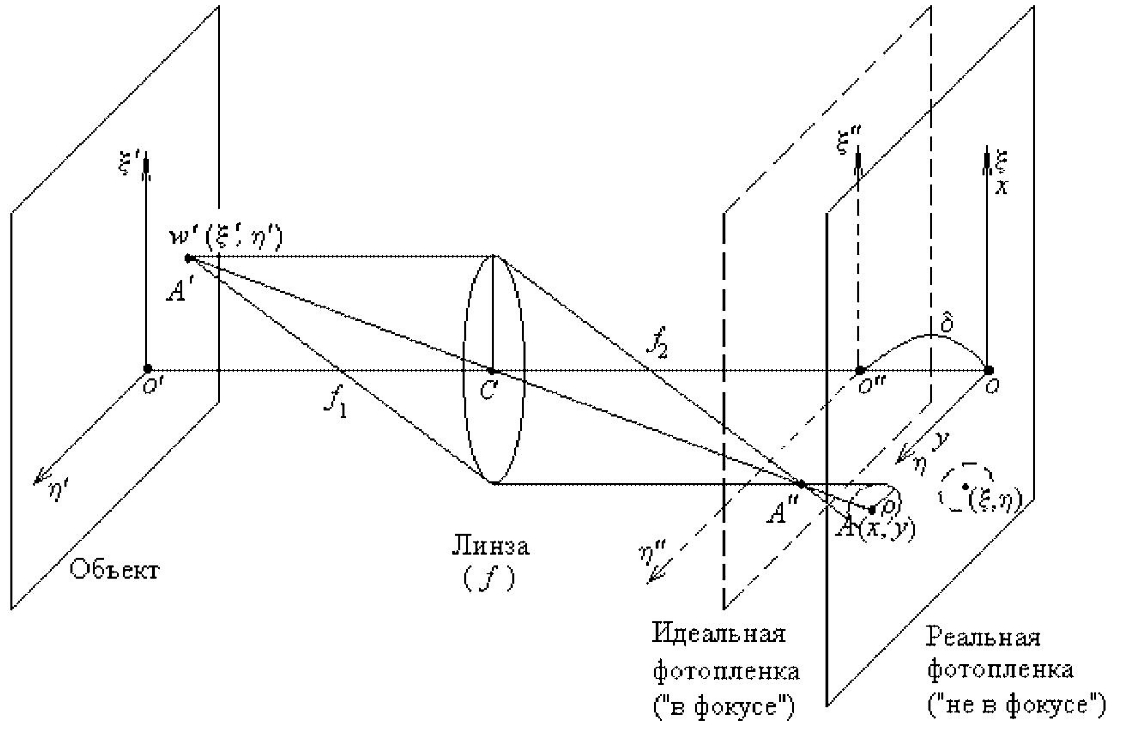
\includegraphics[scale=0.5]{assets/schema}}
	\caption{Принцип получения расфокусированного изображения}
\end{figure}

Пусть снимаемый объект, полагаемый плоским из-за его удаленности, и фотопленка (или матрица сенсоров) расположены параллельно тонкой линзе по разные стороны от нее. 

Пусть $f_1$ --- расстояние от линзы до объекта, а $f_2$ --- расстояние от линзы до фотопленки (матрицы), установленной в <<фокусе>>, а $\sigma$ --- погрешность фокусировки изображения. Таким образом, реальная фотопленка установлена <<не в фокусе>>.

Как видно из рисунка, лучи из точки $A'$ после их прохождения через линзу отобразятся на реальной фотопленке не в точку, а в некоторое размытое пятно, определяемое т.~н. функцией размытия точки, или функцией искажения ядра.~\cite{schema2}

%Соответственно при использовании фотоаппарата изображение будет расфокусированным, если неправильно настроен фокус камеры.

\clearpage

\section*{Вывод}

Для получения восстановленного изображения необходимо произвести обратные вычисления, однако деконволюция (операция, обратная свертке) математически очень трудоемкая и нетривиальная операция. Вследствие этого были разработаны методы восстановления, решающие поставленную задачу иными способами.
\chapter{Конструкторский раздел}

В данном разделе сформулированы требования и ограничения к разрабатываемому методу. Разработан метод восстановления дефокусированных изображений на основе определенных параметров искажения. Описаны основные этапы разработки в виде детализированной диаграммы IDEF0 и схем алгоритмов, а также изложены особенности излагаемого метода. Спроектировано программное обеспечение для реализации разрабатываемого метода.

\section{Требования и ограничения к разрабатываемому методу}

К методу восстановления дефокусированных изображений на основе определенных параметров предъявляются следующие требования:

\begin{enumerate}
	\item Определять параметр искажения (радиус дефокусировки).
	\item Определять функцию рассеяния точки, которая была применена к искаженному изображению.
	\item Восстанавливать искаженное изображение с использованием ФРТ.
\end{enumerate}

Также представлен ряд ограничений для разрабатываемого метода:

\begin{enumerate}
	\item Качество восстановления может быть неудовлетворительным, если изображение было подвергнуто существенному сжатию.
	\item Качество восстановления может быть неудовлетворительным, если изображение с высоким уровнем шума и/или имеет высокочастотные детали (выбросы интенсивности).
\end{enumerate}

Не предполагается обработка изображений c частичной дефокусировкой, т.е. когда искажение присутствует только в определенной области, а не распространяется на всю площадь. Для обработки дефокусировки в этом случае можно выделить часть необходимую изображения. Не предполагается обработка заведомо недефокусированных изображений. Не предполагается повторое применение метода к изображению.

Также естественным ограничением семейства методов деконволюции (как <<слепой>>, так и классической) является тот факт, что чем сильнее искажение (больше радиус дефокусировки), тем менее эффективен метод, т.к. дефокусировка является лишь частично обратимым процессом. Это связано с тем, что при увеличении силы влияния искажения теряется снижается количество информации на изображении.

\section{Требования к разрабатываемому программному обеспечению}

К разрабатываемому программному обеспечению предъявляются следующие требования:

\begin{enumerate}
	\item Возможность загрузки изображений в формате PNG, JPG или BMP.
	\item Возможность обработки как RGB~--~изображений, так и изображений в тонах серого.
	\item Возможность просмотра результата восстановления в сравнении с исходным изображением.
	\item Возможность сохранения результата в отдельный файл в формате PNG, JPG или BMP.
	\item Если время выполнения программы может превышать комфортное время реакции системы для человека, необходимо обеспечить вывод предупреждающего сообщения. 
	\item Разрабатываемое ПО должно корректно реагировать на любые действия пользователя.
\end{enumerate}

\clearpage

\section{Основные этапы разрабатываемого метода}

\subsection{IDEF-0 диаграмма уровня А1}

На рисунке \ref{idef0-a1} представлена диаграмма IDEF0 уровня А1 для разрабатываемого метода.

\begin{figure}[H]
	\centering
	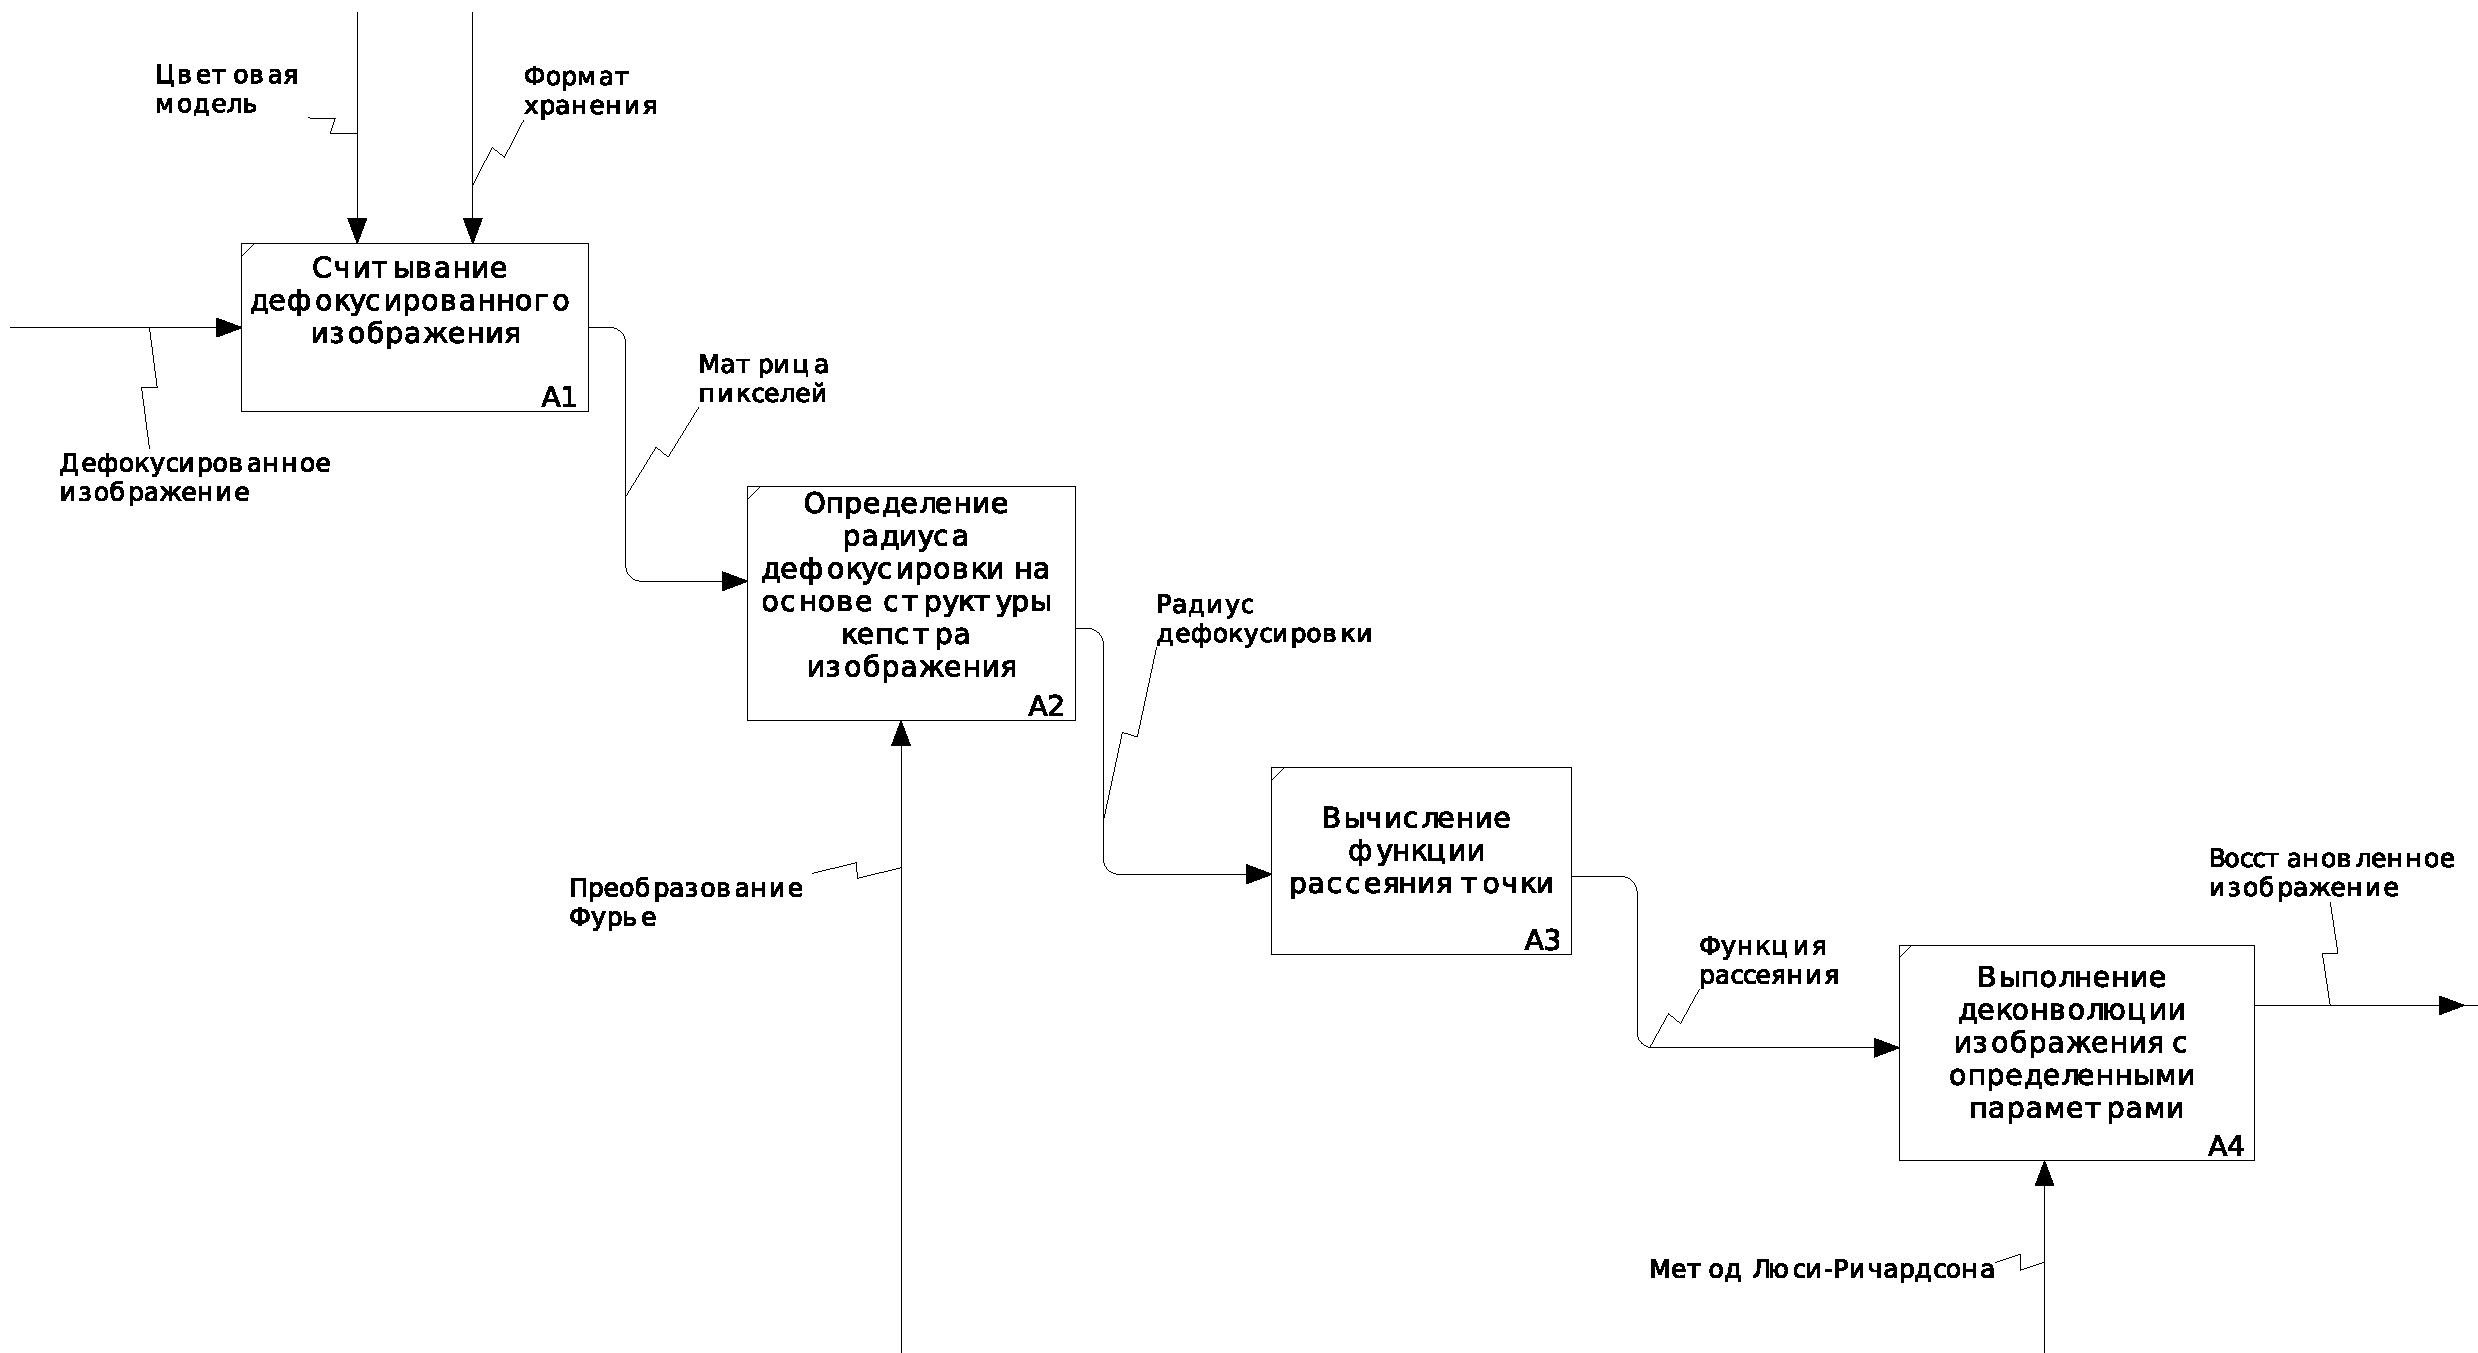
\includegraphics[scale=0.4]{assets/02_A0}
	\caption{IDEF0~--~диаграмма уровня А1}
	\label{idef0-a1}
\end{figure}

\subsection{Схемы алгоритмов} 

На \textit{первом} этапе исходное дефокусированное изображение считывается в матрицу пикселей, с которой в дальнейшем будут происходить все вычисления. В соответствии с требованиями, изображение может одноканальным (grayscale) или трехканальным (RGB). В первом случае все действия производятся однократно, во втором~---~необходимо воспроизвести соответствующие вычисления для каждого из каналов, а затем результат объединить в трехканальное изображение.

На \textit{втором} этапе происходит определение радиуса дефокусировки на основе структуры кепстра изображения. Основная идея предлагаемого метода заключается именно в этом этапе.

На рисунке \ref{r=15} представлена схема, демонстрирующая влияние радиуса на данную структуру. В соответствии с этой закономерностью решено вычислять радиус дефокусировки как отношение радиуса ближайшего к центру кольца к размеру радиального профиля, равного половине ширины изображения.

\begin{figure}[H]
	\centering
	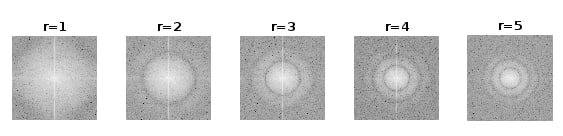
\includegraphics[scale=0.9]{assets/r15.jpg}
	\caption{Влияние радиуса дефокусировки на структуру кепстра изображения}
	\label{r=15}
\end{figure}

На рисунке \ref{cepstrum} представлен алгоритм вычисления кепстра.

\begin{figure}[H]
	\centering
	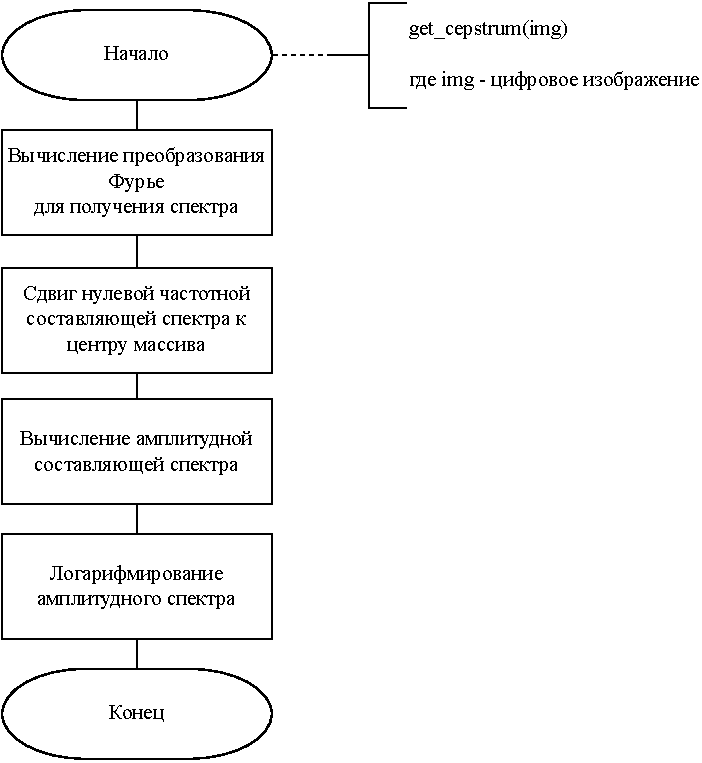
\includegraphics[scale=1]{assets/cepstrum.pdf}
	\caption{Алгоритм вычисления кепстра изображения}
	\label{cepstrum}
\end{figure}

Сдвиг нулевой частотной составляющей необходим для удобства восприятия полученной структуры. Логарифмирование кепстра производится также с целью повышения качества визуального восприятия. Для получения амплитудной составляющей необходимо вычислить модуль кепстра. %обратное ПФ нужно ли?

На рисунке \ref{radius} представлен алгоритм вычисления радиуса дефокусировки на основе кепстрального анализа.

\begin{figure}[H]
	\centering
	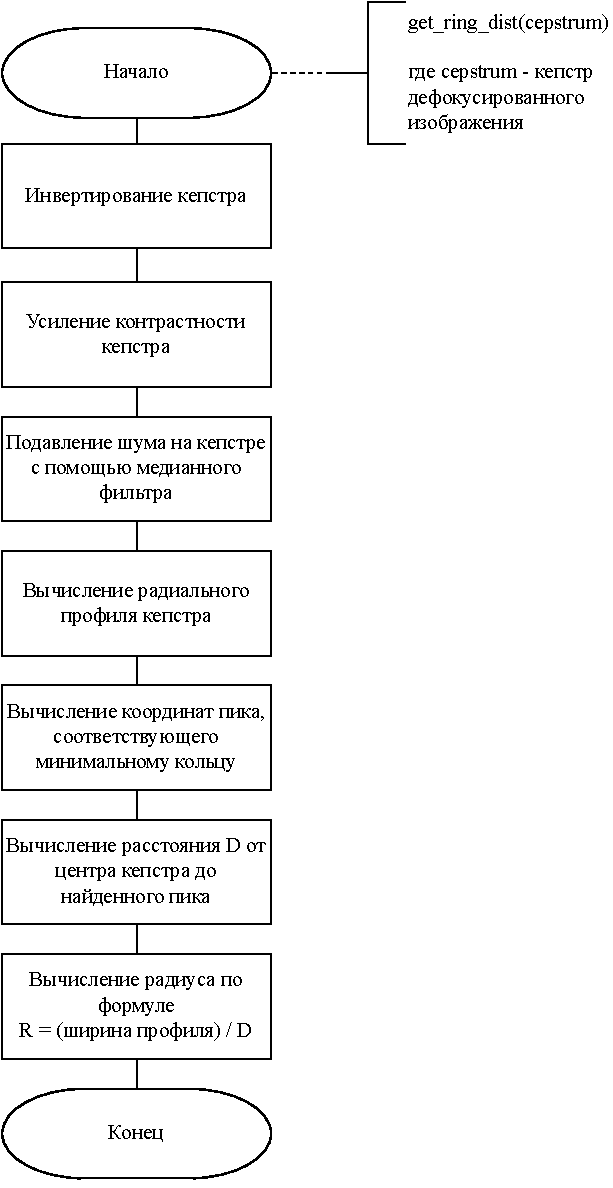
\includegraphics[scale=0.9]{assets/radius.pdf}
	\caption{Алгоритм вычисления радиуса дефокусировки}
	\label{radius}
\end{figure}

В рамках этого этапа входным параметром является матрица пикселей, выходным --- радиус дефокусировки.

Инвертирование кепстра выполняется по причине того, что большинство средств обработки сигналов предоставляет широкий набор обработки пиков (максимумов) интенсивности. 

Усиление контрастности проводится с целью повышения точности распознавания радиуса кольца кепстра. 

Применение медианного фильтра позволяет подавить шум на изображении, сгладив помеху типа <<соль~-~перец>> в центре кепстра. Размер окна выбран так, чтобы не потерять информацию о деталях наблюдаемой структуры.

На \textit{третьем} этапе метода составляется функция рассеяния точки, описывающая процесс искажения, на основе определенного на предыдущем этапе радиуса дефокусировки. Данная матрица имеет тип квадратной матрицы размером, равным радиусу. 

В данный квадрат вписан круг радиусом, также равным двойному радиусу дефокусировки. Для ячеек матрицы, принадлежащих этому кругу, значение интенсивности вычисляется как $\cfrac{1}{\pi r^2}$, где $r$ --- радиус. Для остальных ячеек матрицы значение интенсивности равно 0.

На рисунке \ref{disk} представлен общий вид функции рассеяния точки.

\begin{figure}[H]
	\centering
	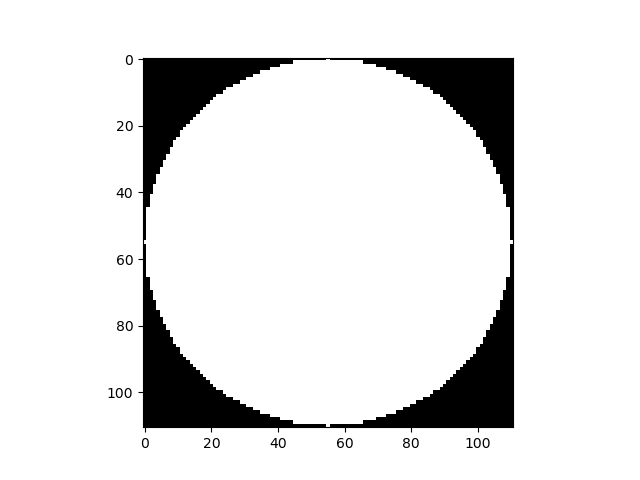
\includegraphics[scale=0.7]{assets/disk.png}
	\caption{Общий вид ФРТ}
	\label{disk}
\end{figure}

В рамках этого этапа входным параметром является радиус дефокусировки, выходным --- квадратная матрица пикселей, описывающая ФРТ заданного радиуса.

\clearpage

На рисунке \ref{psf} представлен алгоритм вычисления ФРТ на основе радиуса.

\begin{figure}[H]
	\centering
	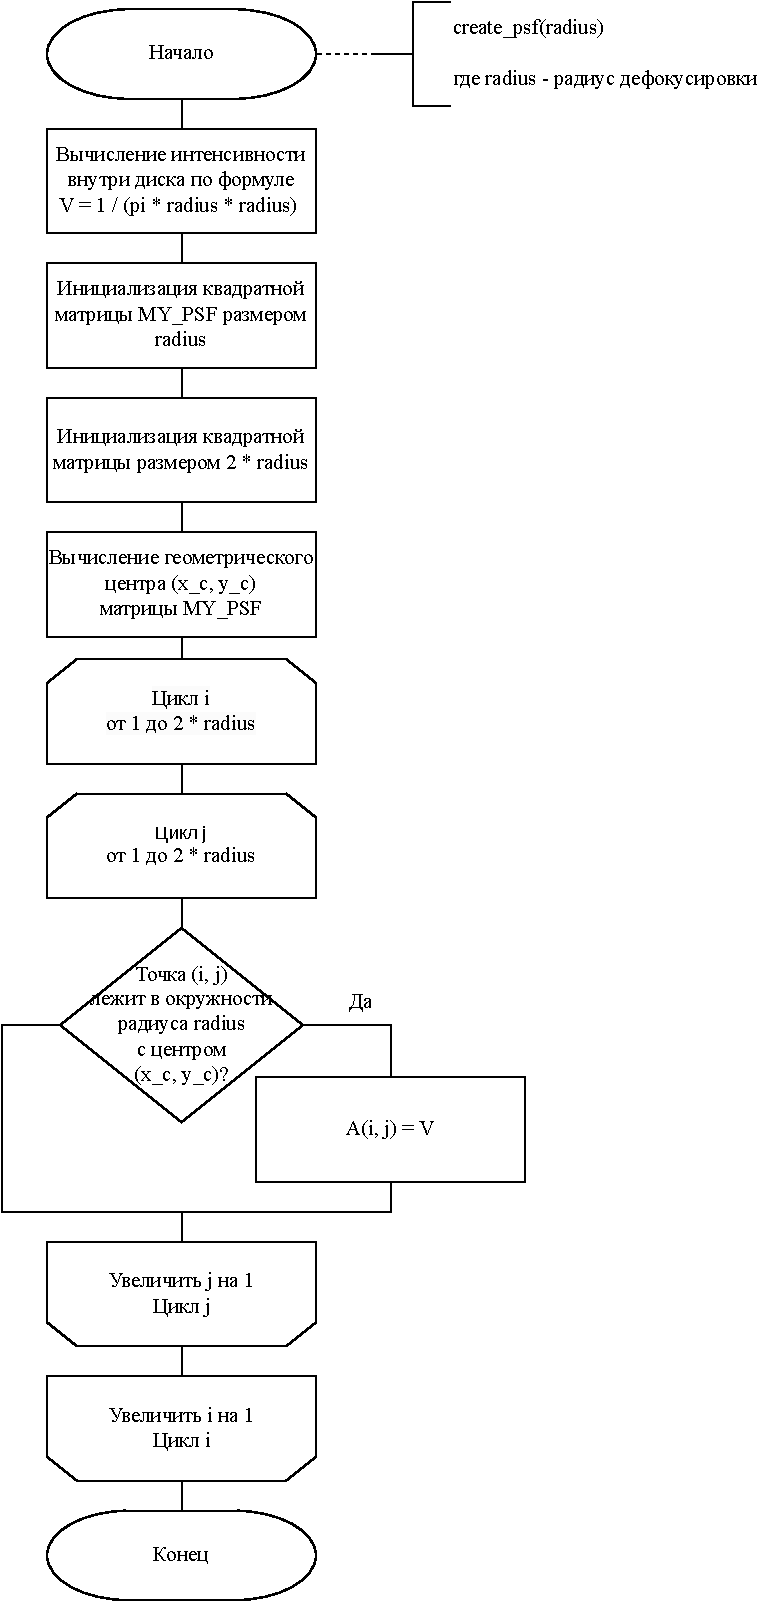
\includegraphics[scale=0.82]{assets/psf.pdf}
	\caption{Алгоритм вычисления ФРТ на основе радиуса дефокусировки}
	\label{psf}
\end{figure}

На \textit{четвертом} этапе производится деконволюция с использованием априорной информации методом Люси~---~Ричардсона. Т.к. этот алгоритм является классическим и не является объектом исследования, было принято решение не останавливаться подробно на реализации этого алгоритма.

На рисунке \ref{deconvolve} представлен алгоритм классической деконволюции на основе определенных параметров искажения.

\begin{figure}[H]
	\centering
	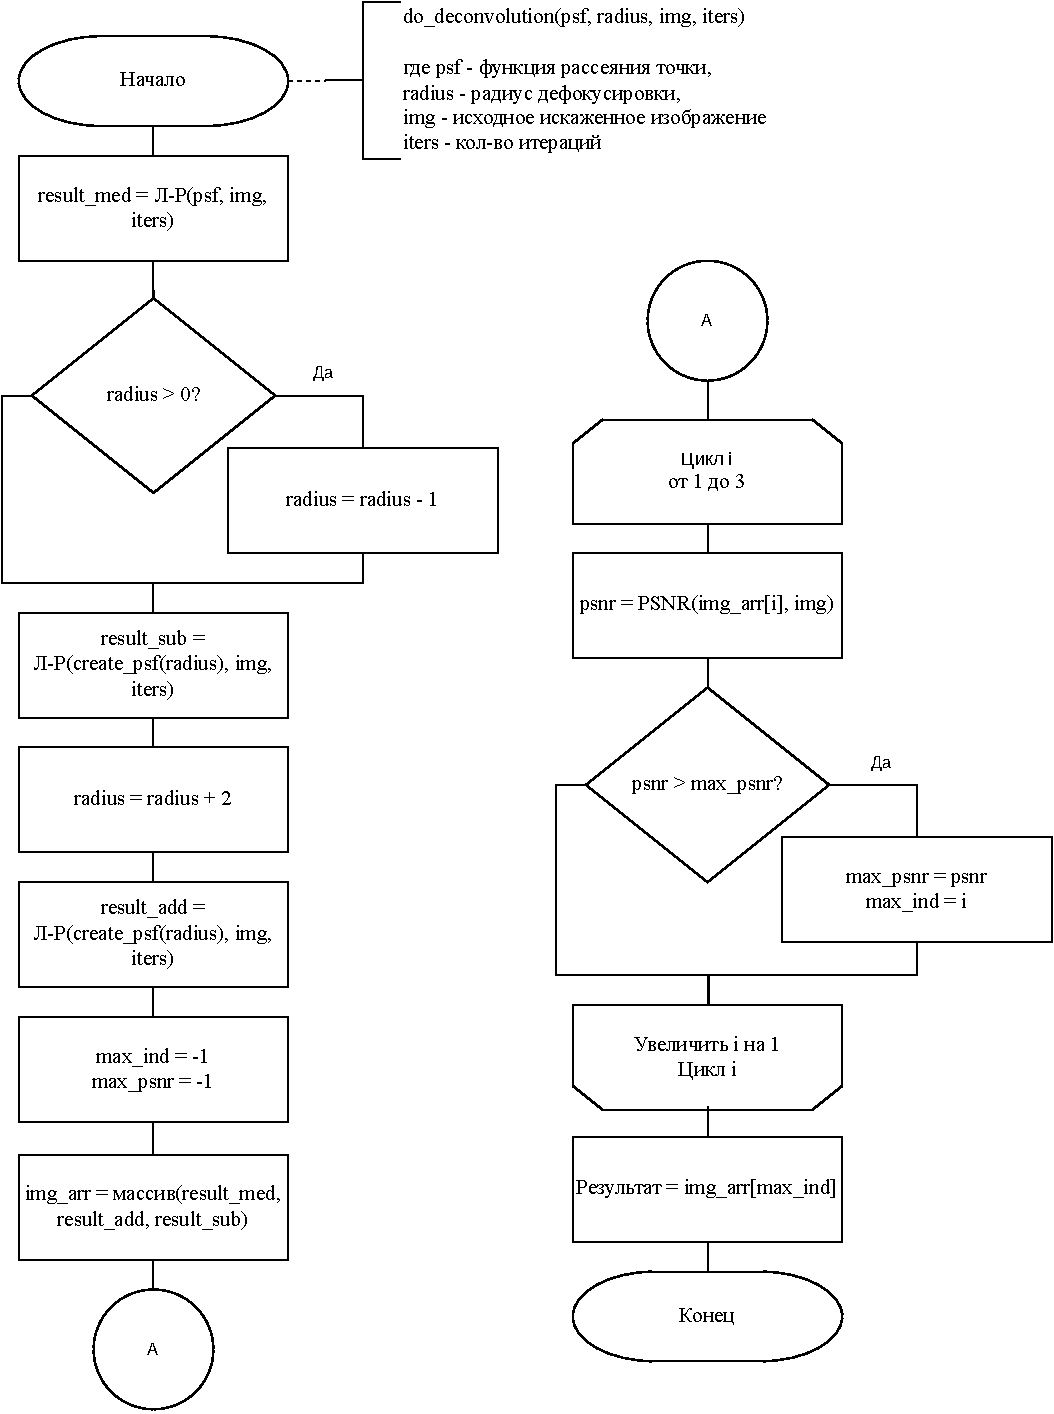
\includegraphics[scale=0.8]{assets/deconvolve.pdf}
	\caption{Алгоритм классической деконволюции на основе определенных параметров искажения}
	\label{deconvolve}
\end{figure}

Также было предложено варьировать на единицу в большую и меньшую сторону радиус дефокусировки, т.к. из-за наличия шума присутствует вероятность ошибиться на несколько пикселей с точностью вычисления радиуса. 

Для выбора наилучшего приближения из трех было предложено использовать метрику <<пиковое соотношение сигнал~--~шум>> (англ. PSNR --- Peak Signal Noise Ratio). Чем больше значение этой метрики, тем лучше произошло восстановление по предположению.

В рамках заключительного этапа входными параметрами являются радиус дефокусировки, ФРТ и исходное изображение, выходным --- матрица пикселей, соответствующая восстановленному изображению.

\subsection{Структура разрабатываемого программного обеспечения}

На рисунке \ref{struct} представлена диаграмма компонентов разрабатываемого программного обеспечения.

\begin{figure}[H]
	\centering
	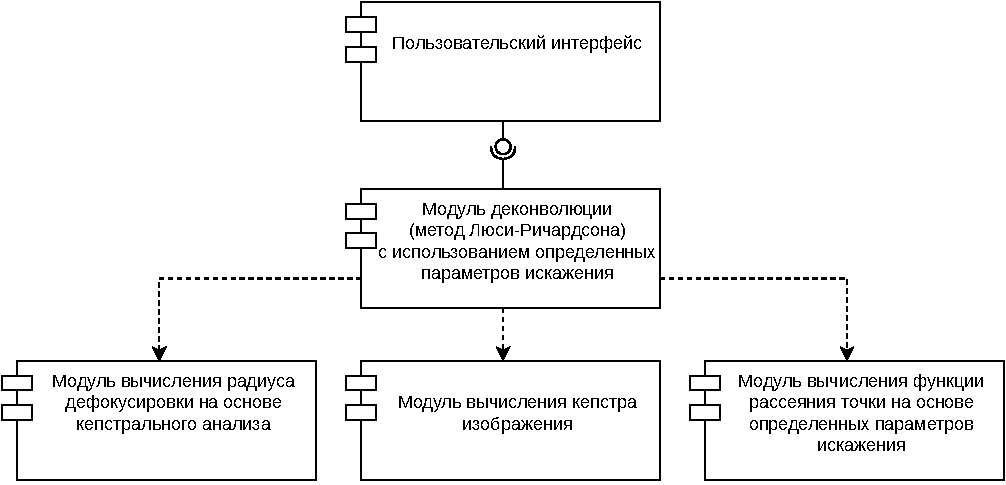
\includegraphics[scale=0.9]{assets/structure.pdf}
	\caption{Диаграмма компонентов разрабатываемого ПО}
	\label{struct}
\end{figure}

\section*{Выводы}

В данном разделе были сформулированы требования и ограничения к разрабатываемому методу и соответствующему ПО, рассмотрены основные этапы разрабатываемого метода в виде детализированной диаграммы IDEF0 и схем алгоритмов, а также спроектирована структура разрабатываемого ПО.
\chapter{Технологический раздел}

В данном разделе обоснован выбор средств программной реализации предлагаемого метода, описан формат входных и выходных данных. Представлены детали реализации метода, а также описано взаимодействия пользователя с программным обеспечением.

\section{Выбор средств реализации программного обеспечения}

\textbf{Выбор языка программирования}

В качестве языка программирования для реализации предлагаемого метода был выбран MatLAB~\cite{matlab_doc}. 

Выбор обусловлен тем, что данный язык имеет широкие возможности для работы с сигналами, для расчета и проектирования аналоговых и цифровых фильтров, для построения их частотных, импульсных и переходных характеристик. 

В наличии также имеются средства для спектрального анализа и синтеза, в частности, для реализации прямого и обратного преобразования Фурье.~\cite{matlab}

\subsection{Выбор среды разработки}

Matlab предоставляет интегрированную среду разработки MatLAB IDE, предоставляющую множество инструментов и функций для разработки, отладки и выполнения кода на MatLAB. Данная среда разработки предоставляет такие компоненты как текстовый редактор, панель переменных окружения, история команд, интеграция файловой системы и др.

\subsection{Используемые расширения}

Для работы с цифровыми изображениями было использовано расширение Image Processing ToolBox~\cite{image_toolbox}, предоставляющее полный набор стандартных алгоритмов и приложений для обработки изображений, анализа, визуализации и разработки новых алгоритмов. Для обработки сигналов --- расширение Signal Processing ToolBox~\cite{signal_toolbox}, предоставляющее функции и интерактивные приложения для анализа, предобработки и выделения признаков из сигналов. Для компиляции приложения в независимый исполняемый файл использовалось расширение MatLAB Compiler~\cite{compiler}.

\section{Формат входных и выходных данных}

Входные данные для разрабатываемого метода:

\begin{itemize}
	\item дефокусированное цифровое изображение в одном из следующих расширений: PNG, JPG или BMP.
\end{itemize}

Выходные данные для разрабатываемого метода:

\begin{itemize}
	\item восстановленное цифровое изображение в одном из следующих расширений: PNG, JPG или BMP.
\end{itemize}

\section{Детали реализации предлагаемого метода}

В листинге 3.1 представлена функция вычисления кепстра изображения.

\begin{lstlisting}[caption={Функция вычисления кепстра изображения}]
function img_cepstrum = cepstrum(img)
	spectrum = fftshift(fft2(img));
	img_cepstrum = log(1+abs(spectrum .* spectrum));
end
\end{lstlisting}

В листинге 3.2 представлена функция вычисления радиуса дефокусировки на основе кепстрального анализа.

\begin{lstlisting}[caption={Функция вычисления радиуса дефокусировки}]
function defocus_radius = radius(cepstrum)
	max_intensity = double(max(cepstrum(:)));
	cepstrum = max_intensity - double(cepstrum);
	cepstrum = medfilt2(cepstrum, [2 2]);
	
	x_c = idivide(int32(size(cepstrum, 1)), 2) + mod(size(cepstrum, 1), 2) + 1;
	central_row = cepstrum(x_c, :);
	half_central_row = central_row(1:size(central_row, 2) / 2);
	half_central_row = flip(half_central_row);
	
	[peaks, peaks_locations] = findpeaks(half_central_row);
	[~, new_peak_locations] = findpeaks(peaks, 'NPeaks', 1);
	defocus_radius = round(x_c / peaks_locations(new_peak_locations));
end
\end{lstlisting}

В листинге 3.3 представлена функция определения функции рассеяния точки на основе вычисленного радиуса фокусировки.

\begin{lstlisting}[caption={Функция определения ФРТ}]
function defocus_psf = psf(radius)
	value = 1 / pi / double(radius) / double(radius);
	
	defocus_psf = zeros(radius * 2, radius * 2);
	
	x_c = radius;
	y_c = radius;
	
	w = radius * 2;
	
	for i = 1:w
		for j = 1:w
			if (i - x_c) * (i - x_c) + (j - y_c) * (j - y_c) <= radius * radius
				defocus_psf(i, j) = value;
			end
		end
	end

end
\end{lstlisting}

\clearpage

В листинге 3.4 представлена функция одноканальной деконволюции на основе метода Люси~--~Ричардсона. Полный вариант функции представлен в приложении A.

\begin{lstlisting}[caption={Функция деконволюции на основе метода Люси~--~Ричардсона}]
function focused_img = my_blind_deconvolution(original_img)
	import cepstrum.*
	import radius.*
	import psf.*

	function img = do_gray()
		img_cepstrum = cepstrum(original_img);
		focus_radius = radius(img_cepstrum);
		focus_psf = psf(focus_radius);
		med_img = deconvlucy(original_img, focus_psf, 100);

		if focus_radius - 1 > 0
			focus_radius = focus_radius - 1;
			focus_psf = psf(focus_radius);
		end
		sub_img = deconvlucy(original_img, focus_psf, 100);
		
		focus_radius = focus_radius + 2;
		focus_psf = psf(focus_radius);
		add_img = deconvlucy(original_img, focus_psf, 100);
		
		psnr_value_med = psnr(med_img, original_img);
		psnr_value_sub = psnr(sub_img, original_img);
		psnr_value_add = psnr(add_img, original_img);
		[~, max_index] = max([psnr_value_med psnr_value_sub psnr_value_add]);

		if max_index == 1
			img = med_img;
		elseif max_index == 2
			img = sub_img;
		else
			img = add_img;
		end
	end
	... % RGB processing
	if length(size(original_img)) == 2
		focused_img = do_gray();
	else
		... % RGB processing
	end
end
\end{lstlisting}

\clearpage

\section{Описание взаимодействия пользователя с программным обеспечением}

На рисунке \ref{gui} представлен разработанный пользовательский интерфейс программного обеспечения.

\begin{figure}[H]
	\centering
	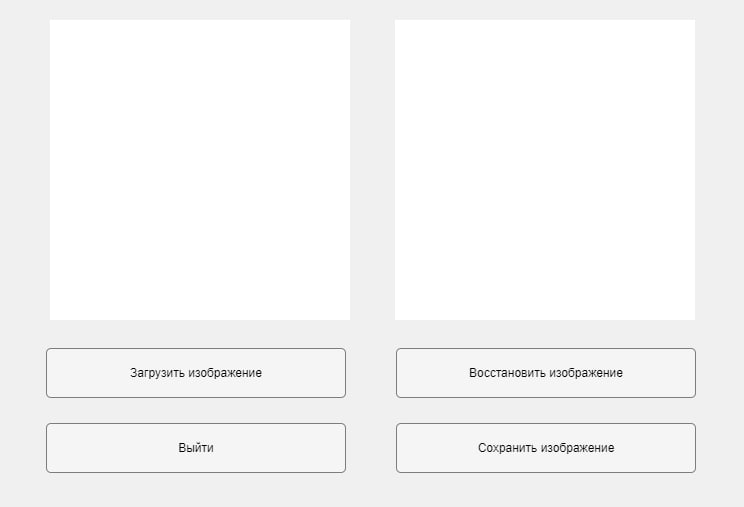
\includegraphics[scale=0.75]{assets/gui}
	\caption{Пользовательский интерфейс программного обеспечения}
	\label{gui}
\end{figure}

Разработанный интерфейс позволяет выбрать исходное цифровое изображение для обработки из файловой системы, применить операцию восстановления к загруженному изображению, а также сохранить полученный результат в отдельный файл.

Процесс выполнения операции восстановления может превышать комфортное время реакции интерактивной системы для человека, в связи с чем при обработке выводится специальное уведомление (рисунок \ref{wait}).

\begin{figure}[H]
	\centering
	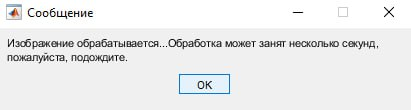
\includegraphics[scale=1]{assets/wait_msg}
	\caption{Уведомление о возможном превышении времени реакции системы}
	\label{wait}
\end{figure}

При попытке восстановить изображение без предварительной загрузки исходного изображения также выводится специальное уведомление для пользователя (рисунок \ref{load}).

\begin{figure}[H]
	\centering
	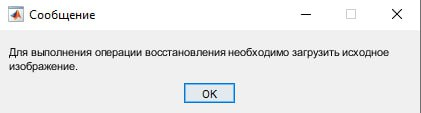
\includegraphics[scale=1]{assets/load_msg}
	\caption{Уведомление о необходимости предварительной загрузки изображения}
	\label{load}
\end{figure}

\section{Сборка и запуск проекта}

В случае, если на персональный компьютер пользователя уже установлен MatLAB, то для сборки и запуска разработанного ПО необходимо выполнить следующие шаги:

\begin{itemize}
	\item проверить наличие компонентов Image Processing Toolbox и Signal Processing Toolbox; 
	\item проверить, что все необходимые файлы и функции, связанные с проектом, находятся в одной папке или в структурированной иерархии папок;
	\item запустить программу MatLAB на компьютере;
	\item открыть папку проекта;
	\item запустить ПО либо через консольный интерфейс (gui.m), либо через соответствующую кнопку <<Run>> в панели инструментов.
\end{itemize}

В случае, если MatLAB не установлен, то необходимо выполнить следующие шаги:

\begin{itemize}
	\item проверить, что исполняемый файл и другие файлы, связанные с проектом, находятся на целевой машине пользователя;
	\item запустить исполняемый файл;
	\item пройти инсталляцию компонента MatLab Runtime~\cite{runtime}, предлагаемую при первом запуске проекта, с целью загрузки минимально необходимого программного обеспечения для запуска проекта без лицензионного экземпляра Matlab; 
	\item запустить проект.
\end{itemize}
\chapter{Исследовательский раздел}

В данном разделе приведены примеры идеального случая восстановления, среднего и плохого. Произведены исследования для определения времени обработки изображения в зависимости от радиуса дефокусировки и цветовой модели, а также полноты решения поставленной задачи. На основе полученных экспериментальных данных сделаны соответствующие выводы.

\section{Технические характеристики}

Технические характеристики машины, на которой производились исследования:

\begin{itemize}
	\item операционная система: Windows 10 64-bit;
	\item оперативная память: 16 Gb;
	\item процессор: AMD(R) Ryzen(TM) 5 4500U CPU @ 2.3 CHz;
	\item количество ядер: 8.
\end{itemize}

\section{Исследование времени работы предложенного метода в зависимости от размера изображения и цветовой модели}

\subsection*{Постановка исследования}

Исследование заключается в определении времени обработки изображения в зависимости от двух факторов: его размера и цветовой модели (трехканальная цветовая RGB~--~модель или одноканальная серая (англ. Grayscale) модель). 

Для замеров должны быть использованы дефокусированные изображения различных размеров и пропорций. Замеры необходимо провести несколько раз для минимизации влияния случайных факторов.

Гипотеза заключается в том, что графики зависимостей будут иметь линейный вид, а также время, затраченное на обработку цветного изображения, будет превышать время обработки одноканального изображения примерно в 3 раза.

\subsection*{Результаты исследования}

В таблице 4.1 представлены результаты замеров времени выполнения алгоритма в зависимости от размера исходного изображения и цветовой модели (RGB~--~модель или Grayscale). Размер изображения измеряется в пикселях, а время --- в секундах. Для замеров времени выполнения использовались команды \textit{tic} и \textit{toc}, представленные в MatLAB.

\renewcommand{\arraystretch}{1.5}
\begin{table}[h!]
	\begin{center}
		\caption{Зависимость времени обработки изображения от его размера и цветовой модели}
		""\newline
		\label{tabl}
		\begin{tabular}{ |c|c|c| } 
			\hline
			\textbf{Размер изображения}, (Ш $\times$ В, пиксели) & \textbf{RGB}, сек. & \textbf{Grayscale}, сек.\\
			\hline
			300 $\times$ 300 & 4.45 & 1.5\\
			\hline
			300 $\times$ 500 & 10.29 & 3.26\\
			\hline
			400 $\times$ 400 & 10.23 & 2.94\\
			\hline
			500 $\times$ 500 & 16.96 & 4.70\\
			\hline
			300 $\times$ 900 & 17.07 & 5.84\\
			\hline
			600 $\times$ 600 & 20.48 & 6.87\\
			\hline
			500 $\times$ 900 & 29.76 & 10.06\\
			\hline
			700 $\times$ 700 & 28.07 & 9.74\\
			\hline
			500 $\times$ 1200 & 40.29 & 13.39\\
			\hline
			700 $\times$ 900 & 42.53 & 14.06\\
			\hline
			800 $\times$ 800 & 37.09 & 13.07\\
			\hline
			900 $\times$ 900 & 49.67 & 16.52\\
			\hline
			700 $\times$ 1200 & 57.75 & 19.35\\
			\hline
			1000 $\times$ 1000 & 62.09 & 20.59\\
			\hline
			1100 $\times$ 1100 & 77.00 & 27.06\\
			\hline
			1200 $\times$ 1200 & 93.28 & 32.32\\
			\hline
		\end{tabular}
	\end{center}
\end{table}

\clearpage

На рисунке \ref{speed} представлена зависимость времени обработки изображения от количества пикселей и используемой цветовой модели.

\begin{figure}[!h]
	\centering
	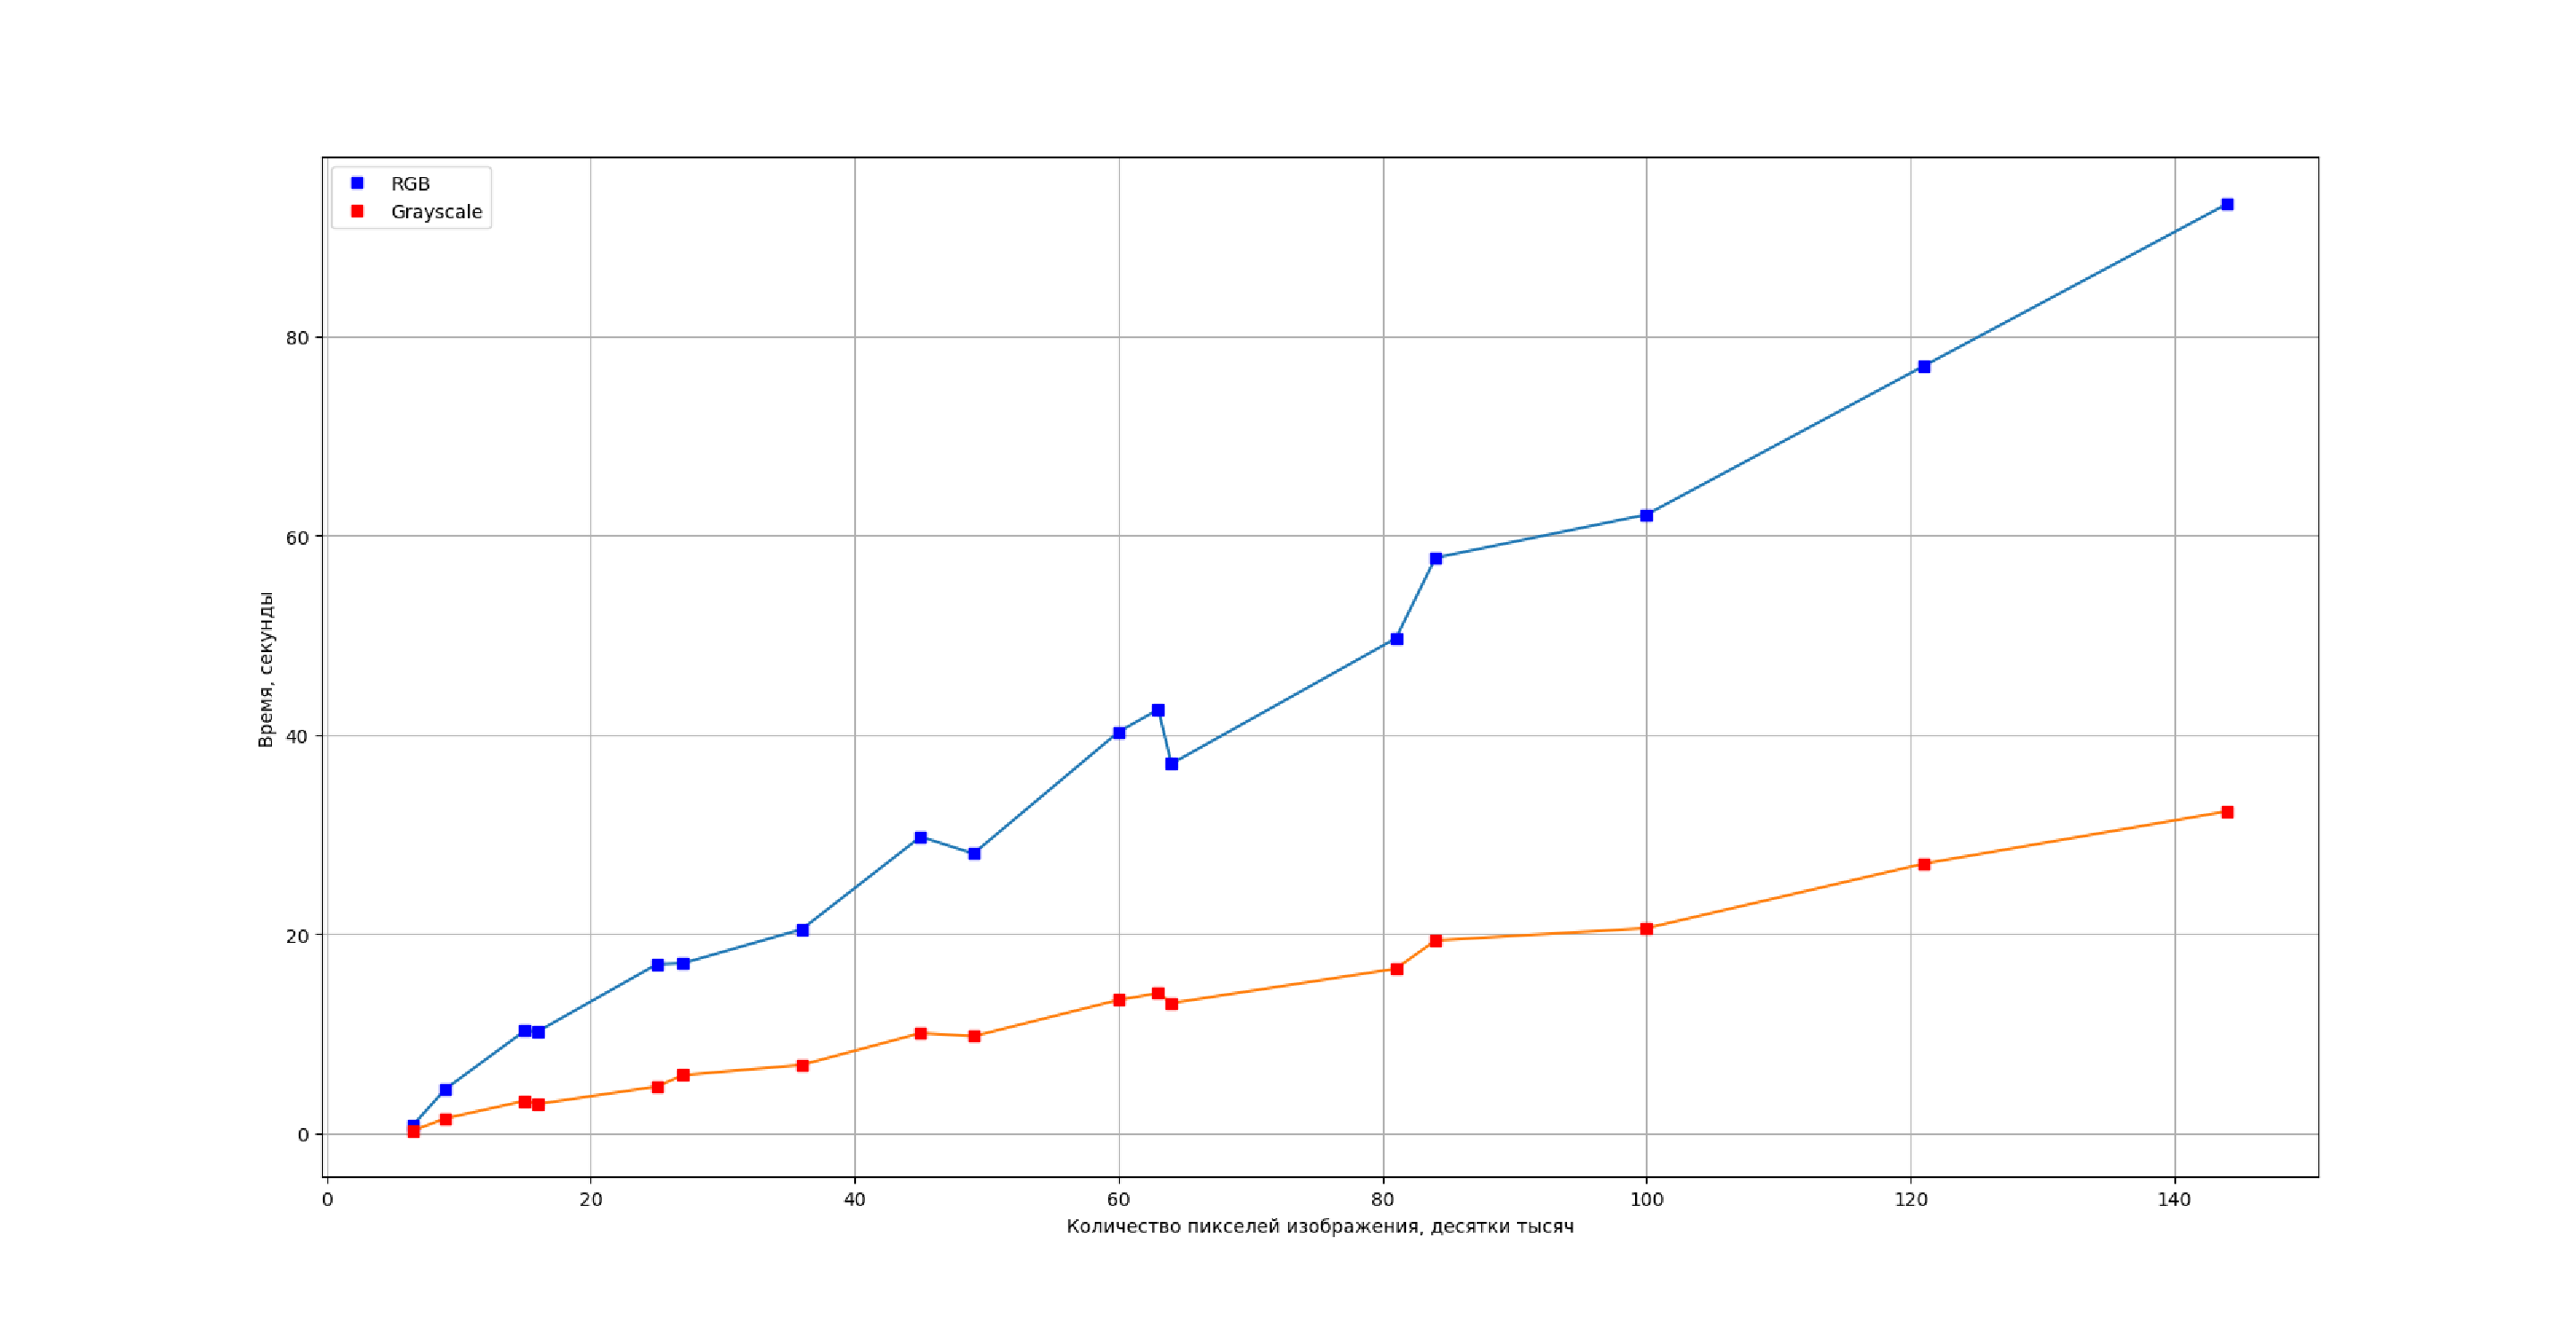
\includegraphics[scale=0.37]{assets/speed}
	\caption{Зависимость времени обработки изображения от количества пикселей и цветовой модели}
	\label{speed}
\end{figure}

Гипотеза подвердилась --- график зависимости имеет линейный вид, а также обработка цветных изображений требует примерно в 3 раза больше времени, чем обработка одноканальных изображений, что подтверждает линейность работы алгоритма относительно аддитивной цветовой модели. 

Таким образом, если цветовая информация об изображении не является критической для рассмотрения, то рекомендуется использовать изображения в тонах серого, т.к. с точки зрения структуры изображения они содержат ту же информацию, однако обработка такого изображения может быть значительно быстрее.

\section{Исследование полноты решения поставленной задачи}

\subsection*{Постановка исследования}

Исследование заключается в определении точности вычисления (в процентах) радиуса дефокусировки в зависимости от его величины и цветовой модели (RGB~--~модель или одноканальная). Для замеров должны быть использованы дефокусированные изображения различных размеров и пропорций.

Гипотеза заключается в том, что при радиусе размытия, равном 0 или 1, точность будет низкая, т.к. на кепстре структуры практически не будут наблюдаться. 

При достижении определенного порогового значения радиуса, которое необходимо установить в результате эксперимента, точность восстановления снова станет низкой, т.к. кольца на структуре кепстра будут сконцентрированы ближе к центру, и, соответственно, будет сложно отличить границу кольца от шума вокруг центра. Между описанными двумя областями значений радиусов точность, по предположению, должна быть удовлетворительной. 

Также предполагается, что точность вычислений для RGB~--~модели будет ниже, чем для серой, т.к. цветные изображения могут быть более подвержены шумам, а также в виду корреляции между каналами и дополнительной сложности вычислений может происходить накопление ошибки.

\subsection*{Результаты исследования}

На рисунке \ref{full} представлена зависимость точности вычисления радиуса дефокусировки от его величины и цветовой модели. Для каждого радиуса размытия обрабатывался ряд изображений различного размера и пропорций, а результат усреднялся.

\begin{figure}[H]
	\centering
	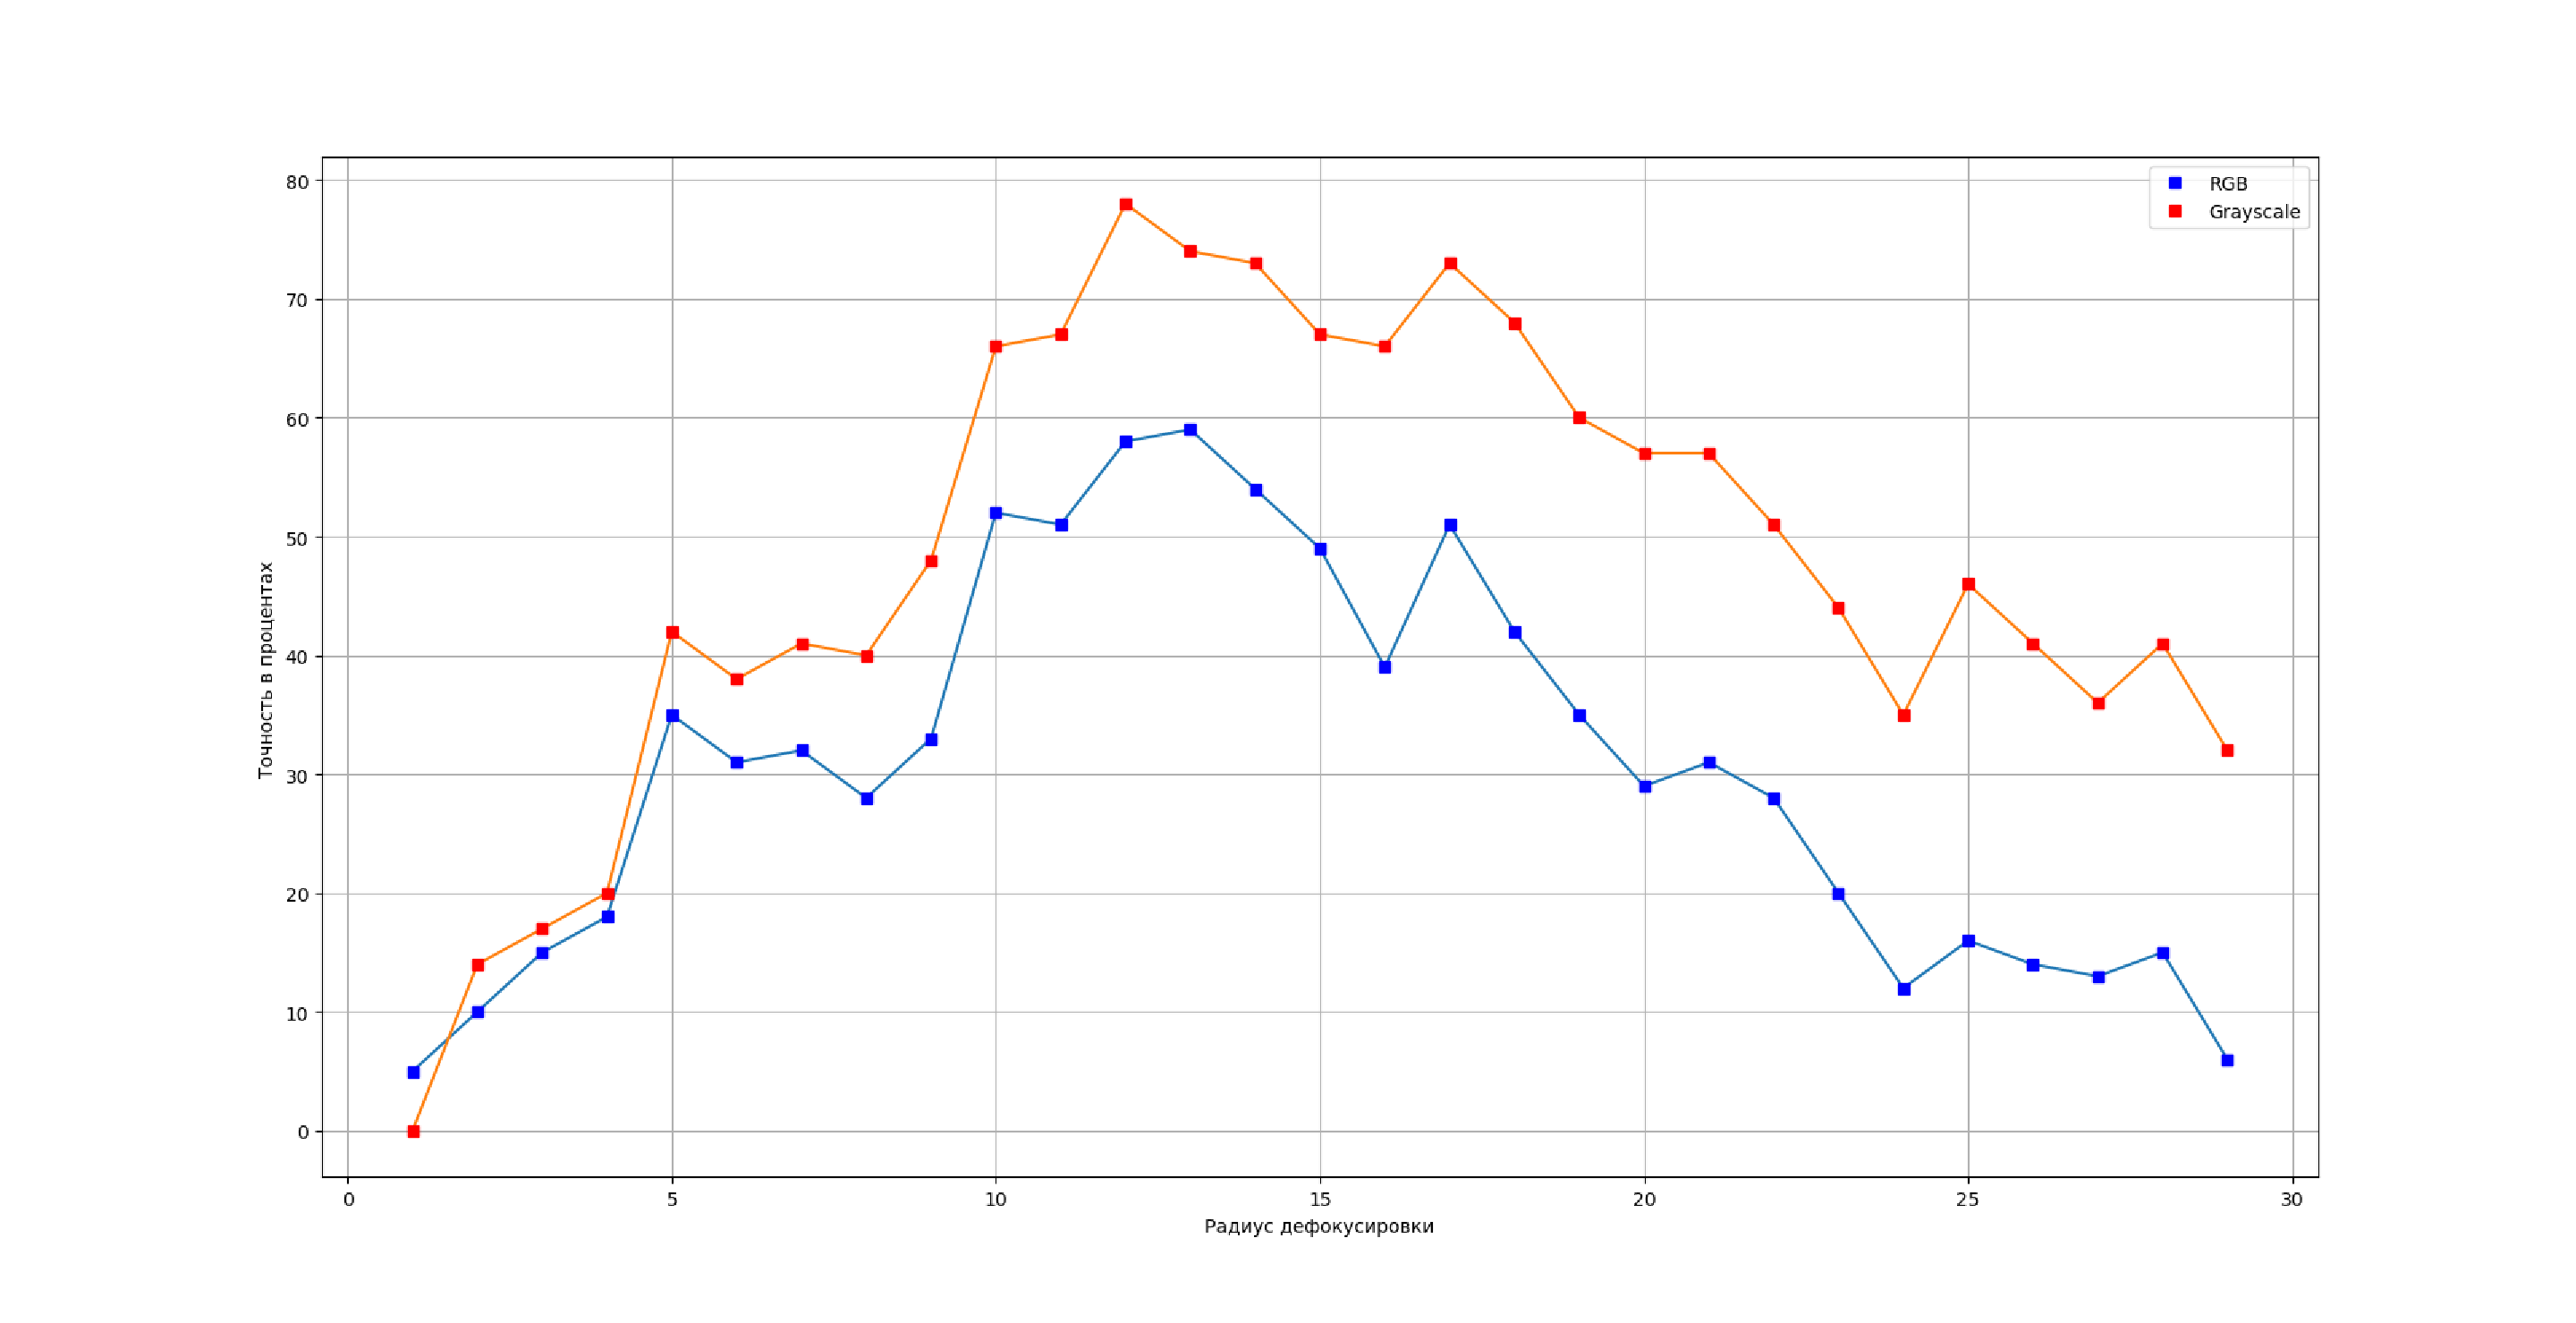
\includegraphics[scale=0.35]{assets/exp_accuracy}
	\caption{Зависимость точности вычисления радиуса дефокусировки от его величины и цветовой модели}
	\label{full}
\end{figure}

В таблице \ref{tabl} представлены результаты исследования полноты полученного решения.

\renewcommand{\arraystretch}{1.3}
\begin{table}[h!]
	\begin{center}
		\caption{Зависимость точности вычисления радиуса дефокусировки от его величины и цветовой модели}
		""\newline
		\label{tabl}
		\begin{tabular}{ |c|c|c| } 
			\hline
			\textbf{Радиус дефокусировки}, пиксели & \textbf{RGB}~--~модель & \textbf{Grayscale}~--~модель\\
			\hline
			0 & 0 \% & 0 \%\\
			\hline
			1 & 5 \%& 0 \%\\
			\hline
			2 & 10 \%& 14 \%\\
			\hline
			3 & 15 \%& 17 \%\\
			\hline
			4 & 18 \%& 20 \%\\
			\hline
			5 & 35 \%& 42 \%\\
			\hline
			6 & 31 \%& 38 \%\\
			\hline
			7 & 32 \%& 41 \%\\
			\hline
			8 & 28 \%& 40 \%\\
			\hline
			9 & 33 \%& 48 \%\\
			\hline
			10 & 52 \%& 66 \%\\
			\hline
			11 & 51 \%& 67 \%\\
			\hline
			12 & 58 \%& 78 \%\\
			\hline
			13 & 59 \%& 74 \%\\
			\hline
			14 & 54 \%& 73 \%\\
			\hline
			15 & 49 \%& 67 \%\\
			\hline
			16 & 39 \%& 66 \%\\
			\hline
			17 & 51 \%& 73 \%\\
			\hline
			18 & 42 \%& 68 \%\\
			\hline
			19 & 35 \%& 60 \%\\
			\hline
			20 & 29 \%& 57 \%\\
			\hline
			21 & 31 \%& 57 \%\\
			\hline
			22 & 28 \%& 51 \%\\
			\hline
			23 & 20 \%& 44 \%\\
			\hline
			24 & 12 \%& 35 \%\\
			\hline
			$\geq$25 & $\leq$20 \%& $\leq$40 \%\\
			\hline
		\end{tabular}
	\end{center}
\end{table}

Для определения точности восстановления в случае одноканальной модели была предложена следующая метрика:

\begin{equation}
	clean\_value = \cfrac{1 - |R_{calc} - R|}{R},
\end{equation}

\begin{equation}
	accuracy = 
	\begin{cases}
		0, & \text{если } clean\_value < 0 \text{ или } |clean\_value| > 1,\\
		clean\_value \cdot 100, & \text{иначе}.
	\end{cases}
\end{equation}

где $accuracy$ --- точность в процентах, $R_{calc}$ --- вычисленный радиус дефокусировки, $R$ --- реальный радиус. Для вычисления среднего значения для каждого радиуса использовалось значение $\cfrac{\sum_{i=1}^{N}accuracy_i}{N}$, где $N$ --- количество замеров. 

С случае оценки точности восстановления цветного изображения метрика $accuracy$ вычислялась для каждого канала независимо, а для получения среднего результата использовалось значение $\cfrac{\sum_{i=1}^{N}r\_accuracy_i\cdot g\_accuracy_i\cdot b\_accuracy_i}{N}$, где $r\_accuracy_i$, $g\_accuracy_i$, $b\_accuracy_i$ --- значение метрики i~--~го замера для красного, зеленого и синего цветовых каналов соответственно.

Таким образом, была определена область применимости предложенного метода: изображения с радиусом дефокусировки в диапазоне от 10 до 20 единиц. 

Если цветовая информация об изображении не является критической для рассмотрения, то рекомендуется использовать изображения в тонах серого, т.к. для этой цветовой модели точность вычислений выше.

\clearpage

\section{Демонстрация вариантов работы метода в зависимости от точности вычислений}

В связи с тем, что разрабатываемый метод основан на методе максимального правдоподобия, возможны несколько классов результатов восстановления: идеальный случай (реальный и вычисленный радиусы совпадают), средний (вычисление радиуса произошло с погрешностью) и плохой случай, когда реальный и вычисленный радиусы существенно не совпадают.

%На рисунке \ref{init} представлено исходное изображение, используемое для проведения эксперимента.
%
%\begin{figure}[H]
%	\centering
%	\includegraphics[scale=0.75]{assets/lena}
%	\caption{Исходное изображение, используемое для проведения эксперимента}
%	\label{init}
%\end{figure}

На рисунках \ref{expr7} и \ref{expr8} представлены примеры высокого (идеального) качества восстановления. Для проведения эксперимента были использованы изображения номера автомобиля~\cite{car} и кота~\cite{cat}.

\begin{figure}[!h]
	\centering
	\begin{subfigure}{.5\textwidth}
		\centering
		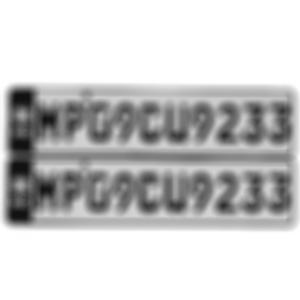
\includegraphics[scale=0.65]{assets/car_perfect}
	\end{subfigure}%
	\begin{subfigure}{.5\textwidth}
		\centering
		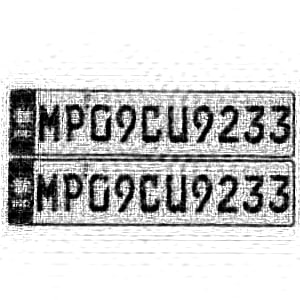
\includegraphics[scale=0.85]{assets/car_perfect_result}
	\end{subfigure}
	\caption{Пример восстановления высокого качества}
	\label{expr7}
\end{figure}

\begin{figure}[!h]
	\centering
	\begin{subfigure}{.5\textwidth}
		\centering
		
\includegraphics[scale=0.45]{assets/cat_perfect}
	\end{subfigure}%
	\begin{subfigure}{.5\textwidth}
		\centering
		
\includegraphics[scale=0.46]{assets/cat_perfect_result}
	\end{subfigure}
	\caption{Пример восстановления высокого качества}
	\label{expr8}
\end{figure}

\clearpage

Пиковое отношение сигнал~--~шум для первой пары изображений составляет 14.7 дб, для второй --- 23 дб.

На рисунках \ref{expr5} и \ref{expr6} представлены примеры среднего качества восстановления. Точность вычисления радиуса дефокусировки составляет $\approx$ 80 процентов.

\begin{figure}[!h]
	\centering
	\begin{subfigure}{.5\textwidth}
		\centering
		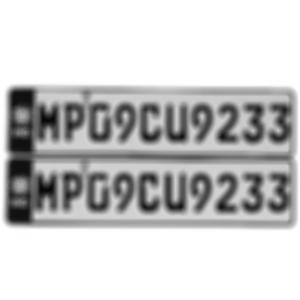
\includegraphics[scale=0.65]{assets/car_r5}
	\end{subfigure}%
	\begin{subfigure}{.5\textwidth}
		\centering
		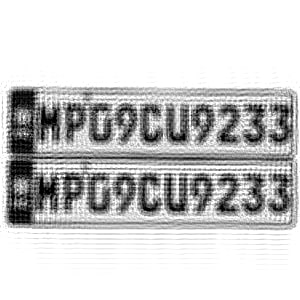
\includegraphics[scale=0.85]{assets/car_r5_result}
	\end{subfigure}
	\caption{Пример восстановления среднего качества}
	\label{expr5}
\end{figure}

\begin{figure}[!h]
	\centering
	\begin{subfigure}{.5\textwidth}
		\centering
		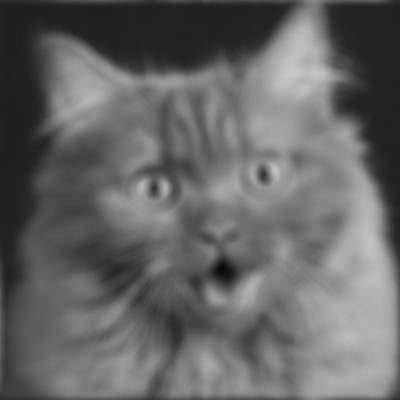
\includegraphics[scale=0.5]{assets/cat_norm}
	\end{subfigure}%
	\begin{subfigure}{.5\textwidth}
		\centering
		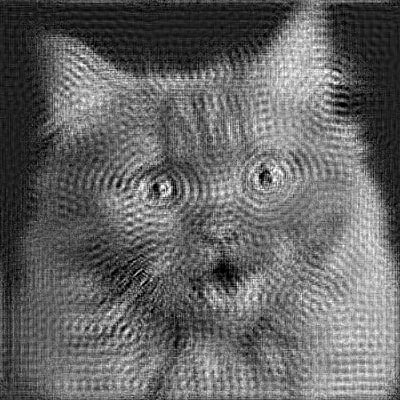
\includegraphics[scale=0.66]{assets/cat_norm_result}
	\end{subfigure}
	\caption{Пример восстановления среднего качества}
	\label{expr6}
\end{figure}

Пиковое отношение сигнал~--~шум для первой пары изображений составляет 19.5 дб, для второй --- 20.22 дб.

\clearpage

На рисунках \ref{expr9} и \ref{expr10} представлены примеры низкого качества восстановления. Точность вычисления радиуса дефокусирвоки составляет $\approx$70 процентов.

\begin{figure}[!h]
	\centering
	\begin{subfigure}{.5\textwidth}
		\centering
		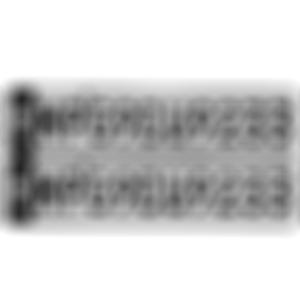
\includegraphics[scale=0.65]{assets/car_bad}
	\end{subfigure}%
	\begin{subfigure}{.5\textwidth}
		\centering
		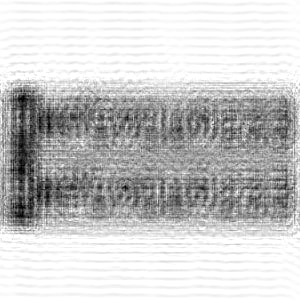
\includegraphics[scale=0.85]{assets/car_bad_result}
	\end{subfigure}
	\caption{Пример восстановления низкого качества}
	\label{expr9}
\end{figure}

\begin{figure}[!h]
	\centering
	\begin{subfigure}{.5\textwidth}
		\centering
		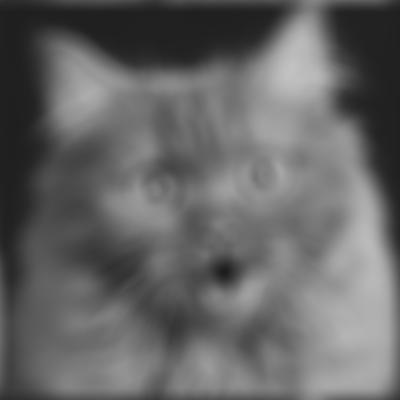
\includegraphics[scale=0.5]{assets/cat_bad}
	\end{subfigure}%
	\begin{subfigure}{.5\textwidth}
		\centering
		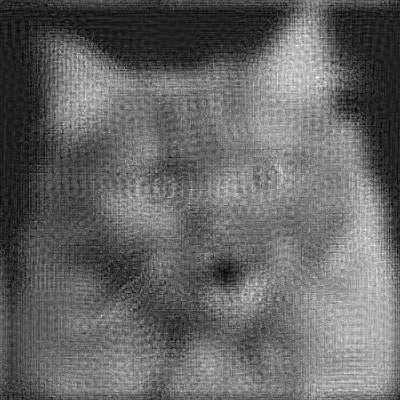
\includegraphics[scale=0.66]{assets/cat_bad_result}
	\end{subfigure}
	\caption{Пример восстановления низкого качества}
	\label{expr10}
\end{figure}

Пиковое отношение сигнал~--~шум для первой пары изображений составляет 21.9 дб, для второй --- 23.8 дб.
%
%\section{Исследование работы метода в случае замыкания}
%
%\subsection*{Постановка эксперимента}
%
%Эксперимент заключается в попытке повторного восстановления изображения, т.е. рассматривается ситуация, когда исходное изображение было для восстановления было получено в результате работы исследуемой программы.
%
%Гипотеза заключается в том, что качество восстановленного повторно изображения станет неудовлетворительным в виду того, что ФРТ для такого изображения будет составлена неверно. Также не будет накапливаться рекуррентная оценка в методе Люси~--~Ричардсона, что приведет к дополнительным артефактам на изображении.
%%, так как сам алгоритм предполагает порождение некоторых артефактов, что при повторном применении приведет к потере информации о деталях изображения и усилении шума
%
%\subsection*{Результаты эксперимента}
%
%На рисунке \ref{exp11} представлен результат первой итерации применения алгоритма.
%
%\begin{figure}[!h]
%	\centering
%	\begin{subfigure}{.5\textwidth}
%		\centering
%		\includegraphics[scale=0.5]{assets/cat_defocused}
%	\end{subfigure}%
%	\begin{subfigure}{.5\textwidth}
%		\centering
%		\includegraphics[scale=0.5]{assets/cat_restored}
%	\end{subfigure}
%	\caption{Результат первой итерации применения алгоритма}
%	\label{exp11}
%\end{figure}
%
%На рисунке \ref{exp12} представлен результат второй итерации применения алгоритма.
%
%\begin{figure}[!h]
%	\centering
%	\begin{subfigure}{.5\textwidth}
%		\centering
%		\includegraphics[scale=0.5]{assets/cat_restored}
%	\end{subfigure}%
%	\begin{subfigure}{.5\textwidth}
%		\centering
%		\includegraphics[scale=0.5]{assets/cat_repeat}
%	\end{subfigure}
%	\caption{Результат второй итерации применения алгоритма}
%	\label{exp12}
%\end{figure}
%
%Таким образом, гипотеза подтвердилась: при замыкании предложенного метода качество восстановления существенно ухудшается. При повторных попытках восстановить изображение методом <<слепой>> деконволюции его качество может ухудшаться по нескольким причинам, таким как накопление ошибки, несовершенство модели искажения, увеличение шума, усиление артефактов.
%
%\clearpage

%\section{Исследование работы предложенного метода в случае восстановления заведомо недефокусированного изображения}
%
%\subsection*{Постановка эксперимента}
%
%Эксперимент заключается в попытке восстановления заведомо недефокусированного изображения.
%
%Гипотеза заключается в том, что качество изображения станет неудовлетворительным.
%
%\subsection*{Результаты эксперимента}
%
%На рисунке \ref{exp12} представлен результат применения алгоритма к заведомо недефокусированному изображению.
%
%\begin{figure}[!h]
%	\centering
%	\begin{subfigure}{.5\textwidth}
%		\centering
%		\includegraphics[scale=0.55]{assets/text}
%	\end{subfigure}%
%	\begin{subfigure}{.5\textwidth}
%		\centering
%		\includegraphics[scale=0.75]{assets/text_restored}
%	\end{subfigure}
%	\caption{Результат применения алгоритма для недефокусированного изображения}
%	\label{exp2}
%\end{figure}
%
%Таким образом, гипотеза подтвердилась.

\section*{Выводы}

Было выявлено, что зависимость времени обработки изображения от его размера и цветовой модели имеет линейный вид, а обработка цветного изображения в среднем требует примерно в 3 раза больше времени, чем обработка серого. 

Была определена область применимости предложенного метода: в диапазоне радиуса дефокусировки от 10 до 20 единиц точность восстановления является удовлетворительный, а в случае обработки серого изображения этот диапазон еще шире, поэтому если учет информации о цвете изображения некритичен, то рекомендуется использовать серое изображение вместо цветного в целях сокращения времени обработки и повышения качества результата. Была описана метрика, используемая для оценки точности.

Были рассмотрены варианты работы программы: идеальный случай, нормальный и плохой, а также проведен анализ значения пикового отношения сигнал~--~шум для каждого варианта. Было выявлено, что метрика PSNR не всегда отражает действительное качество восстановления, т.к. не учитывает психофизиологические особенности восприянтия изображения человеком.
\chapter*{ЗАКЛЮЧЕНИЕ}
\addcontentsline{toc}{chapter}{ЗАКЛЮЧЕНИЕ} 

В данной работе была рассмотрена задача восстановления дефокусированных изображений на основе определенных параметров искажения.

Для достижения поставленной задачи был проведен анализ предметной области дефокусированных изображений, а также существующих методов восстановления без учета априорной информации об искажении. Было выяснено, что функция рассеяния точки в случае дефокусировки фотокамеры имеет форму диска. 

Для решения задачи <<слепой>> деконволюции был предложен метод, согласно которому ФРТ, описывающая искажающий процесс, определялась на основе радиуса колец, которые наблюдаются на структуре кепстра дефокусированных изображений. Также были рассмотрены критерии оценки качества восстановления, основным из которых является пиковое соотношение сигнал~--~шум.

В результате выполнения данной работы было спроектировано и реализовано соответствующее программное обеспечение, позволяющее пользователю загружать искаженное изображение, применять восстановление к нему и сохранять результат. Таким образом, цель работы достигнута.

Разработанный метод имеет ряд ограничений, однако может быть применим даже в условиях отсутствия априорной информации об искажающем процессе. Согласно исследованиям, область применимости предложенного метода~---~изображения с радиусом дефокусировки от 10 до 20 пикселей. Также было выяснено, что в случае, когда пренебержение цветовой информацией является некритичным, то рекомендуется обрабатывать изображение в тонах серого. %Алгоритм не применим для абсолютно всех размытий и подходит лишь под определенный класс задач.

В качестве перспектив дальнейшего развития можно рассмотреть несколько направлений, таких как учет сложной модели искажения, возникающего в реальных ситуациях помимо моделирования известных ФРТ; улучшение обработки шума на изображении; применение <<слепой>> деконволюции к видеофайлам; развитие комбинированных методов деконволюции, охватывающих более широкую область применения; учет частичной дефокусировки.

% % Список литературы при помощи BibTeX
% Юзать так:
%
% pdflatex rpz
% bibtex rpz
% pdflatex rpz

\bibliographystyle{gost780u}
\bibliography{rpz}

%%% Local Variables: 
%%% mode: latex
%%% TeX-master: "rpz"
%%% End: 


\begin{appendices}
\chapter{Полный код функции слепой деконволюции}

В листингах А.1 - А.3 представлен полный код функции слепой деконволюции.

\begin{lstlisting}[caption={Функция слепой деконволюции}]
function focused_img = my_blind_deconvolution(original_img)
	import cepstrum.*
	import radius.*
	import psf.*
	
	function img = do_gray()
		img_cepstrum = cepstrum(original_img);
		focus_radius = radius(img_cepstrum);
		focus_psf = psf(focus_radius);
		med_img = deconvlucy(original_img, focus_psf, 100);
		
		if focus_radius - 1 > 0
			focus_radius = focus_radius - 1;
			focus_psf = psf(focus_radius);
		end
		sub_img = deconvlucy(original_img, focus_psf, 100);
		
		focus_radius = focus_radius + 2;
		focus_psf = psf(focus_radius);
		add_img = deconvlucy(original_img, focus_psf, 100);
		
		psnr_value_med = psnr(med_img, original_img);
		psnr_value_sub = psnr(sub_img, original_img);
		psnr_value_add = psnr(add_img, original_img);
		
		[~, max_index] = max([psnr_value_med psnr_value_sub psnr_value_add]);
		
		if max_index == 1
			img = med_img;
		elseif max_index == 2
			img = sub_img;
		else
			img = add_img;
		end
	end	
\end{lstlisting}
\clearpage
\begin{lstlisting}[caption={Функция слепой деконволюции (продолжение)}]
	function channel_radius = get_radius(channel)
		channel_cepstrum = cepstrum(channel);
		channel_radius = radius(channel_cepstrum);
	end
 
	function focused_channel = apply_psf(channel, radius)
		chanel_focus_psf = psf(radius);
		focused_channel = deconvlucy(channel, chanel_focus_psf, 100);
	end
	
	function img = deconvolve_with_radiuses(red_channel_radius, green_channel_radius, blue_channel_radius)
		red_channel_focused = apply_psf(red_channel, red_channel_radius);
		green_channel_focused = apply_psf(green_channel, green_channel_radius);
		blue_channel_focused = apply_psf(blue_channel, blue_channel_radius);
		img = cat(3, red_channel_focused, green_channel_focused, blue_channel_focused);
	end
	
	function update_radiuses_neg()
		if (red_channel_radius - 1) ~= 0
			red_channel_radius = red_channel_radius - 1;
		end
		if (green_channel_radius - 1) ~= 0
			green_channel_radius = green_channel_radius - 1;
		end
		if (blue_channel_radius - 1) ~= 0
			blue_channel_radius = blue_channel_radius - 1;
		end
	end
	
	function update_radiuses_pos()
		red_channel_radius = red_channel_radius + 2;
		green_channel_radius = green_channel_radius + 2;
		blue_channel_radius = blue_channel_radius + 2;
	end
	
	if length(size(original_img)) == 2
		focused_img = do_gray();
	else
		red_channel = original_img(:, :, 1);
		green_channel = original_img(:, :, 2);
		blue_channel = original_img(:, :, 3);		
\end{lstlisting}
\clearpage
\begin{lstlisting}[caption={Функция слепой деконволюции (продолжение)}]
		red_channel_radius = get_radius(red_channel);
		green_channel_radius = get_radius(green_channel);
		blue_channel_radius = get_radius(blue_channel);
		
		med_rgb_img = deconvolve_with_radiuses(red_channel_radius, green_channel_radius, blue_channel_radius);
		
		update_radiuses_neg();
		sub_rgb_img = deconvolve_with_radiuses(red_channel_radius, green_channel_radius, blue_channel_radius);
		
		update_radiuses_pos();
		add_rgb_img = deconvolve_with_radiuses(red_channel_radius, green_channel_radius, blue_channel_radius);
		
		rgb_psnr_value_med = psnr(med_rgb_img, original_img);
		rgb_psnr_value_sub = psnr(sub_rgb_img, original_img);
		rgb_psnr_value_add = psnr(add_rgb_img, original_img);
		
		[~, max_index] = max([rgb_psnr_value_med rgb_psnr_value_sub rgb_psnr_value_add]);
		
		if max_index == 1
			focused_img = med_rgb_img;
		elseif max_index == 2
			focused_img = sub_rgb_img;
		else
			focused_img = add_rgb_img;
		end
	end
end
\end{lstlisting}

\end{appendices}
\begin{appendices}
\chapter{}

\end{appendices}

\end{document}